
%%%%%    PREAMBLE     %%%%%
% Basics
\documentclass[11pt,twoside]{report}
\usepackage{type1cm}
\usepackage[utf8]{inputenc}
\usepackage[english]{babel}
\usepackage{a4}
\usepackage{float}
\usepackage{lastpage}
\usepackage{amsmath} 
\usepackage[section]{placeins} % Package til \FloatBarrier så man kan styre floats ([section] inkludere automatisk \FloatBarrier i alle sections)
\usepackage[table]{xcolor}
\usepackage{umoline}		   % Package til \Overline{text} .. husk case sensitive !
\usepackage[small]{caption}
%\usepackage{microtype}

%farve til tabler
\usepackage[table]{xcolor}
\usepackage{colortbl}
%\usepackage{kpfonts}

% Indhold -> Indholdsfortegnelse, Bilag -> Appendiks
\addto\captionsdanish{
	\renewcommand\appendixname{Appendix}
	\renewcommand\contentsname{Table of contents}
}
%\usepackage{alnumsec} % Giver mulighed for at bruge \alnumsecstyle{L}, se http://ctan.mackichan.com/macros/latex/contrib/alnumsec/alnumsec.pdf
%\surroundLetter{}{}
\usepackage{appendix}

% Fjerner mellemrum efter , i equations
\usepackage{icomma}

% Giver mulighed for at inkludere pdf'er
%\usepackage{pdfpages}

% Overhold standarder for SI-enheder
\usepackage[%
    %decimalsymbol=comma,                   % Komma som tusindtalsseperator (not anymore!)
    per-mode=fraction,                     % Brug fraction ved fx \meter\per\second (ellers bruger den ms^{-1})
    exponent-product=\cdot,                % Brug \cdot ved videnskabelig notation, fx 21\cdot 10^{3} (ellers bruger den \times)
    complex-root-position = before-number, % Sæt kompleks-del foran tallet
    output-complex-root = \text{j},        % Brug j for kompleks notation
    %output-exponent-marker = \text{e}     % Brug 21e3 i stedet for 21\cdot 10^3
    group-digits = true,                    % Lille mellemrum som tusindtalsseperator
    binary-units = true
    ]{siunitx}
% ex:
%  $\SI{10}{\kilo\ohm}$ svarer til $10\:\text{k}\Omega$
%  Lille si er kun til enheder, fx: \si{\kilo\ohm}
\newcommand{\SIf}[2]{ % \SI med lille fraction (god til in-line stuff)
    %\SI[fraction-function=\slfrac]{#1}{#2}
    \SI[per-mode=symbol]{#1}{#2}
}

% Giver mulighed for at anvende Decibel i SI funktionen
\DeclareSIUnit{\decibel}{dB}
\DeclareSIUnit{\decibelm}{dBm}
\DeclareSIUnit{\decibeli}{dBi}

% Giver adgang til \singlespacing, \doublespacing, og \onehalfspacing
\usepackage{setspace}
% Halvanden linjeafstand (se også software.tex)
\onehalfspacing

% Fjern indents!
%\setlength{\parindent}{0in}

% Afstand mellem caption og teksten nedenunder
%\setlength{\belowcaptionskip}{10pt}
%\setlength{\textfloatsep}{5pt plus 1.0pt minus 2.0pt}
%\setlength{\floatsep}{5pt plus 1.0pt minus 2.0pt}
%\setlength{\intextsep}{5pt plus 1.0pt minus 2.0pt}
% Standard in articles:
%\textfloatsep: 20.0pt plus 2.0pt minus 4.0pt;
%\floatsep: 12.0pt plus 2.0pt minus 2.0pt;
%\intextsep: 12.0pt plus 2.0pt minus 2.0pt.
%\setlength{\abovecaptionskip}{-2ex}
%\setlength{\belowcaptionskip}{-2ex}

% Margins
\usepackage{vmargin}
%\setmargrb{2cm}{1cm}{3cm}{2cm} % Ligesom nedenstående, bare til PS
%\setmargrb{2cm}{1cm}{3cm}{2cm} % Ligesom udskrift, bare med plads til warnings i margin
\setmargrb{2.5cm}{3cm}{2.5cm}{2cm} % Optimal til udskrift! {Venstre/Ryg}{Top}{Højre/Ud}{Bund}

% Billeder
\usepackage{graphicx}
%\usepackage{epstopdf}
\graphicspath{{figures/}}
\usepackage[usenames,dvipsnames]{pstricks}
\usepackage{epsfig}
\usepackage{pst-grad} % For gradients
\usepackage{pst-plot} % For axes
\usepackage{pst-circ} % For circuits
\usepackage{pst-func} % For functions
\psset{gridcolor=lightgray,subgridcolor=white}


% References laves til links
\usepackage{hyperref}
\hypersetup{ 				% Borders omkring links fjernes
	pdfborder = {0 0 0}
}

% Pænere headers og footers
\usepackage{fancyhdr}
\setlength{\headheight}{14pt}
\fancyhf{} % clear header and footer and let me choos myself
% NOTE: http://timmurphy.org/2010/08/07/headers-and-footers-in-latex-using-fancyhdr/
\chead{\leftmark}
\cfoot{\thepage}
% Pænere chapter headings
%\usepackage[Conny]{fncychap}
\usepackage[Lenny]{fncychap}

% Redefiner "Lenny" så der ikke kommer så meget topmargin v. chapter headings
% Originale styles: ftp://cam.ctan.org/tex-archive/macros/latex/contrib/fncychap/fncychap.sty
\makeatletter
\ChNameVar{\fontsize{14}{16}\usefont{OT1}{phv}{m}{n}\selectfont}
  \ChNumVar{\fontsize{60}{62}\usefont{OT1}{ptm}{m}{n}\selectfont}
  \ChTitleVar{\Huge\bfseries\rm}
  \ChRuleWidth{1pt}
  \renewcommand{\DOCH}{%
  	\vspace*{-3cm}                           %flytter kapitel navn op
    \settowidth{\px}{\CNV\FmN{\@chapapp}}
    \addtolength{\px}{2pt}
    \settoheight{\py}{\CNV\FmN{\@chapapp}}
    \addtolength{\py}{1pt}

    \settowidth{\mylen}{\CNV\FmN{\@chapapp}\space\CNoV\thechapter}
    \addtolength{\mylen}{1pt}
    \settowidth{\pxx}{\CNoV\thechapter}
    \addtolength{\pxx}{-1pt}

    \settoheight{\pyy}{\CNoV\thechapter}
    \addtolength{\pyy}{-2pt}
    \setlength{\myhi}{\pyy}
    \addtolength{\myhi}{-1\py}
    \par
    \parbox[b]{\textwidth}{%
    \rule[\py]{\RW}{\myhi}%
    \hskip -\RW%
    \rule[\pyy]{\px}{\RW}%
    \hskip -\px%
    \raggedright%
    \CNV\FmN{\@chapapp}\space\CNoV\thechapter%
    \hskip1pt%
    \mghrulefill{\RW}%
    \rule{\RW}{\pyy}\par\nobreak%
    \vskip -\baselineskip%
    \vskip -\pyy%
    \hskip \mylen%
    \mghrulefill{\RW}\par\nobreak%
    \vskip \pyy}%
    \vskip 20\p@}
 

  \renewcommand{\DOTI}[1]{                   % Chapters m. chapter headings
    \raggedright
    \CTV\FmTi{#1}\par\nobreak
    \vskip 20\p@} %\vskip 40\p@}             % 40->20=mindre afstand mellem chaptername og tekst

  \renewcommand{\DOTIS}[1]{                  % Chapter uden chapter headings
  	\vspace*{-3cm}                           % flytter kapitel navn op
    \raggedright
    \CTV\FmTi{#1}\par\nobreak
    \vskip -20\p@} %\vskip 40\p@}            % 40->-20=mindre afstand mellem chaptername og tekst 
\makeatother

% Nemmere multirow-cells i tabeller
\usepackage{multirow}

% Nemmere multi kolonner
\usepackage{multicol}

% Matematik
\usepackage{amsmath,amsfonts,amssymb}
\newcommand{\slfrac}[2]{\left.#1\middle/#2\right.} % frac med slash
\usepackage{xfrac}

% Placer flere figurer ved siden af hinanden
\usepackage[center]{subfigure}

% Farver på tabeller
\usepackage{colortbl}
\usepackage{array}
\definecolor{lightgray}{RGB}{220,220,220}
\definecolor{lightergray}{RGB}{250,250,250}
\definecolor{jgray}{RGB}{130,130,130}
\definecolor{darkgray}{RGB}{40,40,40}
\definecolor{darkred}{RGB}{136,0,21}
\definecolor{darkblue}{RGB}{0,4,183}
\definecolor{darkerred}{RGB}{110,0,20}
\definecolor{darkgreen}{RGB}{0,160,0}
\definecolor{darkgreen2}{RGB}{16,100,36}
\definecolor{pink}{rgb}{1.,0.75,0.8}
\definecolor{lightblue}{RGB}{153,217,234}
\definecolor{lightyellow}{RGB}{255,255,128}
\definecolor{lightred}{RGB}{255,128,128}
\definecolor{lightpurple}{RGB}{204,0,204}
\definecolor{purple}{RGB}{128,0,128}
\definecolor{sand}{RGB}{245,240,220}
\definecolor{coolblue}{RGB}{0,128,255}


\renewcommand\arraystretch{1.2} % Sæt row height i tabeller

% Giver adgang til \begin{verbatimtab}[8] som viser indents i verbatim environments
\usepackage{moreverb}
\usepackage{fancyvrb}
\usepackage{relsize} % font size som \relsize{2}, relativt til alm fontsize

% Custom commands defineres
% Nemmere figurer, syntaks:
% \fig[keepaspectratio=true,height=40mm]{image}{Teksten til billledet}{billedelabel}
\newcommand{\fig}[4][width=40mm]{
	\begin{figure}[h!]
		\centering
	    \includegraphics[#1]{#2}
	    \caption{#3}
	    \label{#4}	
		%\end{centering}
	\end{figure}
}

\newcommand{\figuc}[4][width=40mm]{
	\begin{figure}[h!]
	    \includegraphics[#1]{#2}
	    \caption{#3}
	    \label{#4}	
	\end{figure}
}

\newcommand{\pfig}[3]{
	\begin{figure}[h!]
		\centering
	    #1
	    \caption{#2}
	    \label{#3}	

	\end{figure}
}

\newcommand{\pcapfig}[4]{
	\begin{figure}[h!]
		\centering
	    #1
	    \caption[#2]{#3}
	    \label{#4}	
	\end{figure}
}

% Nemmere referencer, syntaks:
% \figref{labelpåfigur}         --> figur 3.4 (s. 23)
% \secref{labelpåsektion}       --> sektion 2.7 (s. 7)
% \chref{labelpåchapter}        --> kapitel 2 (s. 4)
% \tref{labelpåtabel}           --> tabel 7.4 (s. 45)
% \cref{labelpåkode}            --> kodeudsnit 8.3 (s. 76)
% \bilref{labelpåbilag}         --> bilag 2.3 (s. 25)
\usepackage{nameref} % Giver adgang til \nameref

%\newcommand{\figref}[1]{figure \ref{#1} (p. \pageref{#1})}
%\newcommand{\Figref}[1]{Figure \ref{#1} (p. \pageref{#1})}
%\newcommand{\secref}[1]{section \ref{#1} (p. \pageref{#1})}
%\newcommand{\Secref}[1]{Section \ref{#1} (p. \pageref{#1})}
%\newcommand{\chref}[1]{chapter \ref{#1} (p. \pageref{#1})}
%\newcommand{\tref}[1]{table \ref{#1} (p. \pageref{#1})}
%\newcommand{\cref}[1]{code snippet \ref{#1} (p. \pageref{#1})}
%\newcommand{\bilref}[1]{annex (Se oversigt, chap. \ref{#1} (p. \pageref{#1}))}
%\newcommand{\equref}[1]{equation \ref{#1} (p. \pageref{#1})}
%\newcommand{\apref}[1]{appendix \ref{#1} (p. \pageref{#1})}
\newcommand{\figref}[1]{figure \vref{#1}}
\newcommand{\Figref}[1]{Figure \Vref{#1}}
\newcommand{\secref}[1]{section \vref{#1}}
\newcommand{\Secref}[1]{Section \Vref{#1}}
\newcommand{\chref}[1]{chapter \ref{#1}}
\newcommand{\tref}[1]{table \vref{#1}}
\newcommand{\cref}[1]{code snippet \vref{#1}}
\newcommand{\anref}[1]{annex (See list, chap. \ref{#1} (p. \pageref{#1}))}
\newcommand{\equref}[1]{equation \vref{#1}}
\newcommand{\apref}[1]{appendix \vref{#1}}
\newcommand{\afigref}[1]{figure \vref{#1}}
\newcommand{\aafigref}[1]{figure \ref{#1}}
\newcommand{\asecref}[1]{section \vref{#1}}
\newcommand{\atref}[1]{table \vref{#1}}
\newcommand{\acref}[1]{code snippet \vref{#1}}
\newcommand{\achref}[1]{chapter \ref{#1} (p. \pageref{#1})}
\newcommand{\aequref}[1]{\vref{#1}}


% Funktion til at få latex til kun at medtage side tal hvis referancen er på en anden side end den der refereres fra
\usepackage{varioref}
\makeatletter
\vref@addto\extrasenglish{%
  \def\reftextfaceafter{(p.~\thevpagerefnum)}
  \def\reftextfacebefore{(p.~\thevpagerefnum)}
  \def\reftextafter{(p.~\thevpagerefnum)}
  \def\reftextbefore{(p.~\thevpagerefnum)}
	\def\reftextfaraway#1{(p.~\thevpagerefnum)}
  \def\reftextcurrent{}
}
\makeatother

% Itemize uden mellemrum mellem linjer
\newenvironment{pitemize}{
\begin{itemize}
  \setlength{\itemsep}{1pt}
  \setlength{\parskip}{0pt}
  \setlength{\parsep}{0pt}
}{\end{itemize}}

% Enumrate uden mellemrum mellem linjer
\newenvironment{penumrate}{
\begin{enumerate}
  \setlength{\itemsep}{1pt}
  \setlength{\parskip}{0pt}
  \setlength{\parsep}{0pt}
}{\end{enumerate}}

% Kommentarer i margen (noter til forfattere)
\usepackage{xkvltxp}
\usepackage[draft]{fixme}
%\usepackage{fixme}       % Skjul margin kommentarer (til udskrift)
% Nemmere kommentarer i margin, syntaks:
%  \note{DitNavn}{Din note}{teksten, noten skal hæftes ved}
% Eks.:
%  Dette er en \note{Tausen}{Hov hov! Du har vist byttet om på kage og gulerødder}{Jeg kan godt lide kage - men gulerødder er nu bedre.} haha - hilsen jesper :D
\newcommand{\note}[3]{
	\fxnote*[author=#1,footnote,nomargin]{#2}{#3}
}

% Til kode-eksempler
\usepackage{color}                        % Package til \color-kommandoen
\usepackage{listings}                     % Package til kodeeksempler
% Caption customization:
%\usepackage{xcolor}
%\usepackage{courier}
%\usepackage{caption}
%\DeclareCaptionFont{white}{\color{white}}
%\DeclareCaptionFormat{listing}{\colorbox{gray}{\parbox{\textwidth}{#1#2#3}}}
%\captionsetup[lstlisting]{format=listing,labelfont=white,textfont=white}
\newcommand{\code}[2]{
  \FloatBarrier
  \lstinputlisting[#1]{#2}
  \FloatBarrier
}

%Ny command til tabler:
%\ptable[scalebox værdi (hvis den bare skal være default skal man ikke have de firkantede parenteser med)]{søjlernes formatering}{
%  tablen uden øverste \hline
%}{caption tekst}{label tekst}
\newcommand{\ptable}[5][0.75]{
  \begin{table}[h!]
    \centering
    %  \rowcolors{2}{lightergray}{}
      \scalebox{#1}{
        \begin{tabular}{#2}
          \hline
          \rowcolor[gray]{0.8}#3
        \end{tabular}
      }
      \caption{#4}
      \label{#5}
    %\end{center}
  \end{table}
}
% Tabeller med notes under, alt andet ligesom ovenstående
% Noterne specificeres som en itemize som sidste parameter:
% \ntable[scalebox]{column format}{table uden første \hline}{caption}{label}{notes}
% ex:
% \ntable{|m{5cm}|}{
%   \textbf{Example table with notes}
%   \hline
%   \hline
%   Row 1\tnote{1} \\
%   \hline
%   Row 2\tnote{2} \\
%   \hline
%   Row 3 \\
%   \hline
% }{
%   \item[1] This is the first row
%   \item[2] And this is the second
% }
\usepackage{threeparttable}
\newcommand{\ntable}[6][0.65]{
  \begin{table}[h!]
    \centering
      \scalebox{#1}{
        \begin{threeparttable}
          \rowcolors{2}{lightergray}{}
          \begin{tabular}{#2}
          #3
          \end{tabular}
          \begin{tablenotes}
            #6
          \end{tablenotes}
        \end{threeparttable}
      }
      \caption{#4}
      \label{#5}
 %   \end{center}
  \end{table}
}

%Ny command til tabler med multirow:
%\ptablemr[scalebox værdi (hvis den bare skal være default skal man ikke have de firkantede parenteser med)]{søjlernes formatering}{
%  tablen uden øverste \hline
%}{caption tekst}{label tekst}
%Derefter skal man selv ind og sætte farve i rækkerne
\newcommand{\ptablemr}[5][0.8]{
  \begin{table}[h!]
    \centering
      \scalebox{#1}{
        \begin{tabular}{#2}
          \hline
          \rowcolor[gray]{0.8}#3
        \end{tabular}
      }
      \caption{#4}
      \label{#5}
  %  \end{center}
  \end{table}
}

%Ny command til tabler til mr. t:
%\ptable[scalebox værdi (hvis den bare skal være default skal man ikke have de firkantede parenteser med)]{søjlernes formatering}{
%  tablen 
%}{caption tekst}{label tekst}
\newcommand{\ptablemrt}[5][0.65]{
  \begin{table}[h!]
    \centering
      \rowcolors{2}{lightergray}{}
      \scalebox{#1}{
        \begin{tabular}{#2}
          #3
        \end{tabular}
      }
      \caption{#4}
      \label{#5}
 %   \end{center}
  \end{table}
}
    
\def\lstlistingname{Code snippet}           % Definerer hvad der står foran et stykke kodes caption
\lstset{
	basicstyle=\footnotesize\ttfamily,    % Lille skrifttype
	keywordstyle=\color{blue}\bfseries,   % Keywords blå og bold
	commentstyle=\color[RGB]{34,139,34},  % Default comments mørkegrøn
	showstringspaces=false,               % Ingen symbol for mellemrum i strings
	numbers=left,                         % Linjenumre til venstre
	numberstyle=\tiny\color{darkgray},    % Små tal på linjenumre med farve skrift
	numbersep=5pt,                        % Afstand fra linjenummer og ind til kode
	backgroundcolor=\color{lightergray},  % Bg farve
	tabsize=2,                            % Indenteringer = 4 spaces
	columns=fixed,                   	  % Kan give problemer med bredde på bogstaver men skulle ikke da vi bruger ttfamily
	breaklines=true,                      % Deler en for lang linje over to linjer
	frame=tb,                		      % Styrer hvor streger skal placeres
	captionpos=t,                         % Caption til kode under og over kodeeksemplet
	rulecolor=\color{black},			  % Farven på frame
	escapeinside={(*@}{@*)},               % Giver mulighed for at lave en (*@\label{label}@*), på en kodelinje,
%										    så man kan referere til linjen
    literate={~}{$\sim$}1 {^}{$\wedge$}1,
}
\lstdefinelanguage{bascom} {              % Definition af BASCOM-language
	classoffset=4,	
	morekeywords={\$regfile,\$crystal,Config, Output, Input, Timer1, Timer0, Do, Loop, If, Then, End, Sub, Wait, Waitms, Declare, As, Int, Word, Byte, Call, And, Or, Else, Until, Goto, Alias, Dim},
		keywordstyle=\color[RGB]{0,0,128}\bfseries,classoffset=3,
	morekeywords={PORTA, PORTB, TCCR1A, TCCR1B, TCCR1C, TCCR1D, TCNT1, OCR1A, OCR1B, OCR1C, OCR1D, PINA, PINB, PINC},
		keywordstyle=\color[RGB]{128,0,0},classoffset=2,
	morekeywords={=, \&, <, >, +, -, *, /, .},
		keywordstyle=\color[RGB]{255,0,0},classoffset=1,
	sensitive=false,
	morecomment=[l]{'},
	commentstyle=\color[RGB]{34,139,34}
}
\lstdefinelanguage{arduino} {              % Definition af ARDUINO-language
	classoffset=4,
	morekeywords={char,int,void,long,
			pinMode,random,available,read,print,millis,digitalWrite,digitalRead,analogWrite,analogRead,delay,
			for,while,switch,break,if,else,bitRead,print,println,begin,return,float,cos,sin,pow,sqrt,bitClear,bitSet,
			true,false},
		keywordstyle=\color[RGB]{204,102,0},classoffset=3,
	morekeywords={setup,Serial,Serial1,Serial2,loop},
		keywordstyle=\color[RGB]{204,102,0}\bfseries,classoffset=2,
	morekeywords={HIGH,LOW,OUTPUT,INPUT},
		keywordstyle=\color[RGB]{0,102,153},classoffset=1,
	sensitive=false,
	morecomment=[l]{//},
	stringstyle=\color[RGB]{0,0,255},
	morestring=[b]",
	morestring=[b]',
	commentstyle=\color[RGB]{50,50,50}
}
\lstdefinelanguage{csharp} {              % Definition af C#-language
	classoffset=3,
	% Variabletypes, keywords
	morekeywords={char,int,void,long,object,string,true,char,false,using,class,
			this,delegate,partial,namespace,
			for,while,switch,break,if,else,new,try,catch,private,public,\#region,\#endregion},
		keywordstyle=\color[RGB]{0,0,255},classoffset=2,
	% Classes
	morekeywords={EventArgs,SerialPortController,StringBuilder,SerialDataReceivedEventHandler,MySqlConnection,
			Exception,MySqlCommand,MySqlDataReader,ConnectionState,PointPairList,ZedGraphControl,Color,
			SymbolType,GraphPane,LineItem,Fill,Size,Point,MethodInvoker,Convert,FormClosedEventArgs,EventArgs,
			SerialPort,StopBits,Parity,Form,Form1},
		keywordstyle=\color[RGB]{43,145,175},classoffset=1,
	sensitive=true,
	morecomment=[l]{//},
	stringstyle=\color[RGB]{163,21,21},
	morestring=[b]",
	morestring=[b]',
	commentstyle=\color[RGB]{0,128,0}
}
\lstdefinelanguage{vhdl} {              % Definition af VHDL-language
	classoffset=4,
	morekeywords={library,use,all,entity,generic,map,architecture,of,is,downto,others,then,if,port,signal,elsif,else,when,for,while,
	              end,process,begin,or,and,not,xor,\&,constant,wait,for,nor,nand,in,out,type,array,with,select,case},
		keywordstyle=\color[RGB]{255,0,0},classoffset=3,
	morekeywords={std_logic,std_logic_vector,to_integer,unsigned,integer,time,natural,1,2,3,4,5,6,7,8,9,0},
		keywordstyle=\color[RGB]{0,145,185},classoffset=2,
    morekeywords={=, <, >, +, -, *, /, .},
		keywordstyle=\color[RGB]{0,0,255},classoffset=1,
	sensitive=true,
	morecomment=[l]{--},
	stringstyle=\color[RGB]{0,145,185},
	morestring=[b]",
	commentstyle=\color[RGB]{0,128,0}
}
\lstdefinelanguage{psm} {              % Definition af PSM(ASM)-language
	classoffset=4,
	morekeywords={and,or,xor,out,in,load,sub,add,comp,call,jump,ret,store,fetch,test,sr0,sr1,sl0,sl1},
		keywordstyle=\color[RGB]{0,0,255},classoffset=3,
	morekeywords={equ,dsout,dsin},
		keywordstyle=\color[RGB]{108,0,117},classoffset=2,
    morekeywords={\$,0,1,2,3,4,5,6,7,8,9},
		keywordstyle=\color[RGB]{0,232,116},classoffset=1,
	sensitive=true,
	morecomment=[l]{;},
	stringstyle=\color[RGB]{0,145,185}
%	morecomment=[l]{\$},
%    commentstyle=\color[RGB]{0,232,116}
}
% TOC settings
\setcounter{tocdepth}{1} % Begræns table of contents til kun 2 niveauer
%\setcounter{tocdepth}{10}
\addtocontents{toc}{\protect\thispagestyle{empty}} % Fjern sidetal fra TOC

% Flowcharts
\usepackage{tikz} 
\newcommand*\circled[1]{\tikz[baseline=(char.base)]{ % circle om tekst
            \node[shape=circle,draw,inner sep=2pt] (char) {#1};}}
\usetikzlibrary{shapes,arrows}
% Define block styles
\tikzstyle{decision} = [diamond, draw=gray, aspect=2, fill=lightgray, text width=2cm, text badly centered, node distance=3cm, inner sep=0pt,minimum height=1cm]
%\tikzstyle{decision} = [regular polygon, regular polygon sides=4, shape border rotate=45, draw, fill=lightgray, text width=1.5cm, text badly centered, node distance=3cm, inner sep=0pt,minimum height=1cm]
\tikzstyle{block} = [rectangle, draw=gray, fill=lightgray, text width=3cm, text centered, minimum height=1cm]
\tikzstyle{endpoint} = [ellipse, draw=gray, fill=lightgray, text width=2cm, text centered, minimum height=1cm]
\tikzstyle{line} = [draw, thick, -latex]

\newcommand{\flowcirc}[1]{
  \psovalbox[fillstyle=solid,fillcolor=lightgray,linecolor=gray]{#1}
}
\newcommand{\flowbox}[1]{
  \psframebox[fillstyle=solid,fillcolor=lightgray,linecolor=gray]{#1}
}
\newcommand{\flowdiamond}[1]{
  \psdiabox[fillstyle=solid,fillcolor=lightgray,linecolor=gray]{#1}
}
\usepackage[square]{natbib}

%%% Stops figures and stuff to float to next section %%%
\usepackage[section]{placeins}
\let\OLDsubsection=\subsection
\renewcommand{\subsection}[1]{\FloatBarrier\OLDsubsection{#1}}
\let\OLDsubsubsection=\subsubsection
\renewcommand{\subsubsection}[1]{\FloatBarrier\OLDsubsubsection{#1}}

% Glossaries
\usepackage[acronym,xindy]{glossaries}
\makeglossaries
\usepackage[xindy]{imakeidx}
\makeindex

\newcommand{\eqdef}{\overset{\mathrm{def}}{=\joinrel=}}

\begin{document}
    \pagenumbering{Roman}
    \singlespacing
    \pagestyle{empty}	
	\begin{center}
	\vspace*{1.5cm}
	
	\begin{Huge}
		\textbf{Mini Project 1\\
		Multi Agent Radio Communication}
	\end{Huge}\\~\\
	
	\vspace*{2cm}
	
	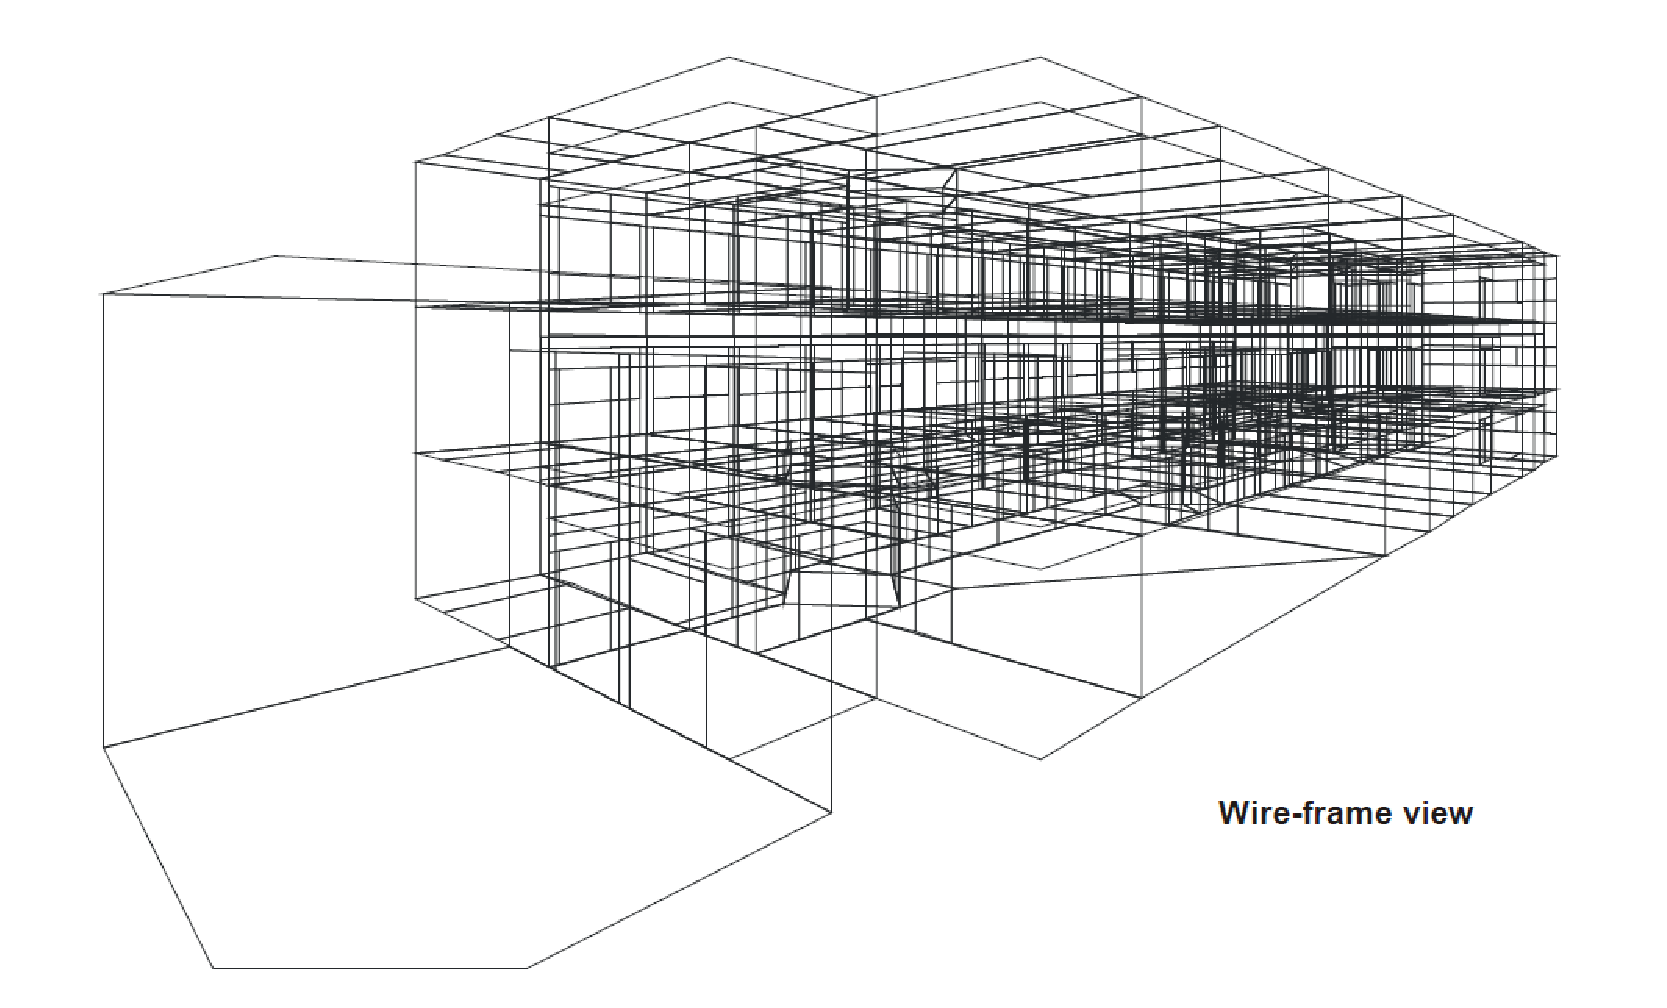
\includegraphics[width=14cm]{FrontPage}
	\center{Mesh sketch of the Novi building}
	\vspace*{2cm}
    
	Aalborg University\\
	P9, Autumn Semester 2014\\
	Wireless Communication Systems\\
\end{center}
	\cleardoublepage
	This paper is the documentation of the work related to the mini-project done in the first part of the course \textit{Multi-Agent Radio Communication}. These mini-project and exercises have been solved and documented as a team effort of the course participants.\\

The group consists of:
	\begin{description}
	\item \hspace{4cm} Jesper Nysted Andersen
 	\item \hspace{4cm} Maria Stefan
 	\item \hspace{4cm} Anders Karstensen
 	\item \hspace{4cm} Maria Carmela Cascino
 	\item \hspace{4cm} Johannes Hejselbæk
 	\item \hspace{4cm} Juan Alberto Cabrera Guerrero
 	\item \hspace{4cm} Djamschid Safi
 	\item \hspace{4cm} Pablo Fuentes
	\end{description}

\vspace{2cm}
The documentation is divided into chapters corresponding to the different exercises of the mini project.
	%\cleardoublepage
	\pagestyle{plain}
		
%%%%% Table of content %%%%%
	\tableofcontents 
	\onehalfspacing
	\pagestyle{fancy} % Normal pagesetup with page numbering (change to plain to remove header)
	\pagenumbering{arabic} 
    \setcounter{page}{0} % Sætter sidetal til 1
%%%%% START OF DOCUMENT  %%%%%	

\part{Patrick Part 1}

\chapter{MM1 - Time reversal techniques}
Advantages of using directive antennas -> space as 4th access/multiplex dimension\\

Beam space vs signal space methods (forward-reverse link sensitivity)\\

User tracking (link) vs traffic tracking (coverage)\\

Access vs interference suppression

\section{Problem A} \label{sec:mm3_PbA}
\textit{MAXIMISING COVERAGE AREA. For a given radiated power, compare the coverage area of a single antenna system, $Ac^1$, to the coverage area of an M-antenna distributed antenna system, $Ac^M$. State the implications of the relation.}\\

We assume, that the minimum acceptable downlink power remains the same for both the single antenna system and the M-antenna system. Also, the total radiated power is constant, so it is divided onto the M antennas. The addition of an index M denotes the belonging to the M-antenna system, so for example $A_c$ is the coverage area of the single antenna system, while $A_{cM}$ is the M-antenna system cell coverage area. 

\begin{flalign}
&& P_{dc} &= P_{dc,M} &\\
&& &=const. &\\
&&\frac{PL}{P_R} &=M \cdot \frac{PL_M}{P_R} &\\
&& PL&=M\cdot PL_M & \label{eq:pathloss_1_M}
\end{flalign}

The relationship between the path loss and the coverage area is given as

\begin{flalign}
PL = C \left(\frac{A_c}{\pi}\right)^\frac{\gamma}{2}. 
\end{flalign}

This can be inserted to \eqref{eq:pathloss_1_M} to find the relation between the coverage area in both cases.

\begin{flalign}
\left(\frac{A_c}{\pi}\right)^{\frac{\gamma}{2}}=M\cdot\left(\frac{A_{cM}}{\pi}\right)^{\frac{\gamma}{2}}\\
A_c^{\frac{\gamma}{2}}=M\cdot (A_{cM})^{\frac{\gamma}{2}}\\
A_c=M^{\frac{2}{\gamma}}\cdot A_{cM} \\
\frac{A_{cM}}{A_{c}} =M^{-\frac{2}{\gamma}} \label{eq:ExpressionForAcWithM} \\
\frac{A_{cM,total}}{A_{c}} =\frac{A_{cM}\cdot M}{A_{c}}=M^{-\frac{2}{\gamma}+1}
\end{flalign}

The implications of this factor are shown in \figref{fig:Acm_M}, \figref{fig:Acmtot_M}, \figref{fig:Acm_gamma}, \figref{fig:Acmtot_gamma} and \figref{fig:Acmtot_gamma_M}. [Additional text to describe implications...?]

\fig[keepaspectratio=true,width=11cm]{Acm_M.eps}{Coverage Area of one cell for multiple antennas vs. antenna number.}{fig:Acm_M}

\fig[keepaspectratio=true,width=11cm]{Acmtot_M.eps}{Total coverage Area for multiple antennas vs. antenna number.}{fig:Acmtot_M}

\fig[keepaspectratio=true,width=11cm]{Acm_gamma.eps}{Coverage Area of one cell for multiple antennas vs. PL coefficient.}{fig:Acm_gamma}

\fig[keepaspectratio=true,width=11cm]{Acmtot_gamma.eps}{Total coverage Area for multiple antennas vs. PL coefficient.}{fig:Acmtot_gamma}

\fig[keepaspectratio=true,width=11cm]{Acmtot_gamma_M.eps}{Total coverage Area vs. PL coefficient and number of antennas.}{fig:Acmtot_gamma_M}



\section{Problem B - SDMA aspect}
\textit{Use the defined antenna patterns/directional signals from exercise A . You would need also some results/idea about exercise A2, if not finished (remember two main tasks : one to find C/I with directional spread signals, other to find shape of full radar sweep (effective antenna pattern wrt user and interferer) and resulting mean direction)}

\subsection{Question 1}
\textit{Now consider a 120 degree sector serviced with above antenna pattern in a SDMA operation (i.e. identical but offset patterns for N users). Consider the system to have power control so all users have same power received at the BS when the individual users antenna pattern maximum is pointed to their respective direction. Assume only a single path from user to BS (like exercise A1))}

\subsubsection{a) For a target C/I=9dB (spatial interference), what is the required user-to-interferer offset angle (to left and right)?. If C/I is 15 dB what then?}

\begin{figure}[!h]
  \centering
  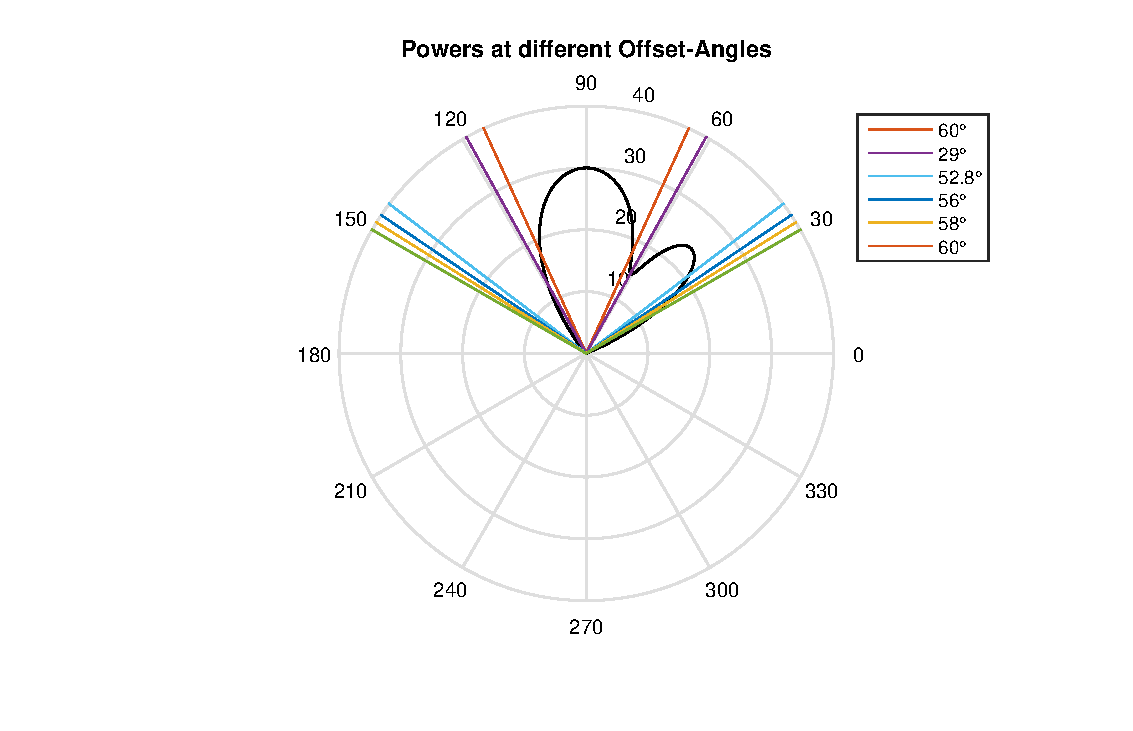
\includegraphics[width=12cm]{offset_angles.eps}
  \caption{Offset angles.}
  \label{fig:offset_angles}
\end{figure}

\begin{figure}[!h]
  \centering
  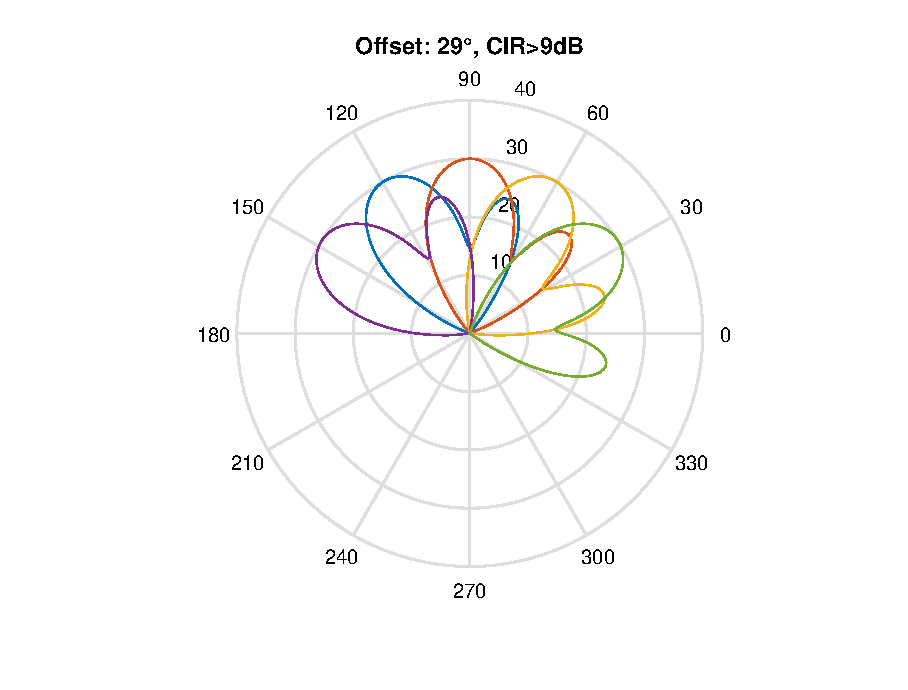
\includegraphics[width=11cm]{offset29deg.eps}
  \caption{Offset 29deg.}
  \label{fig:offset29deg}
\end{figure}

\begin{figure}[!h]
  \centering
  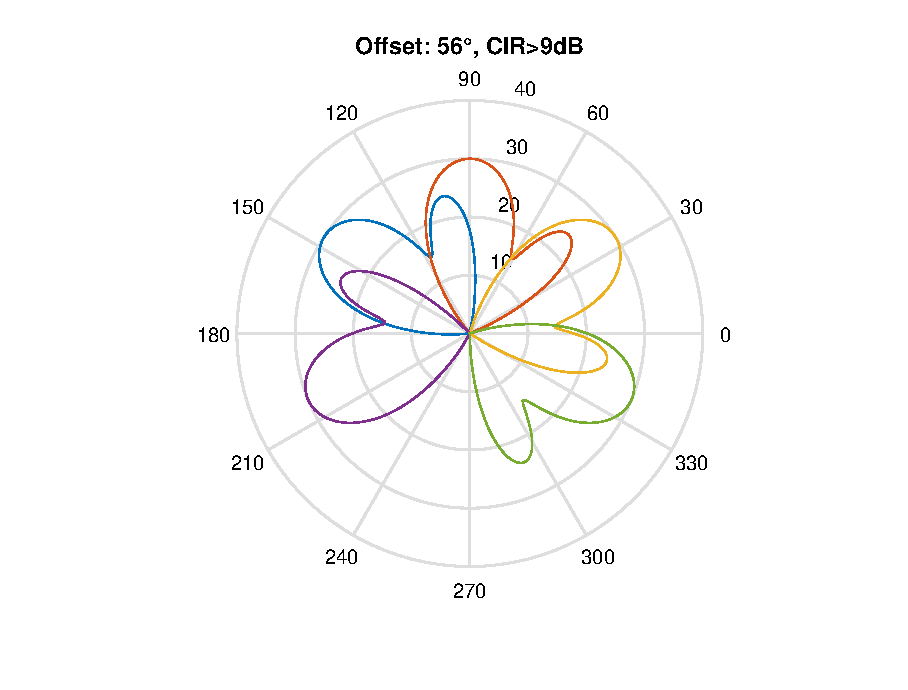
\includegraphics[width=11cm]{offset56deg.eps}
  \caption{Offset 56deg.}
  \label{fig:offset56deg}
\end{figure}

\begin{figure}[!h]
  \centering
  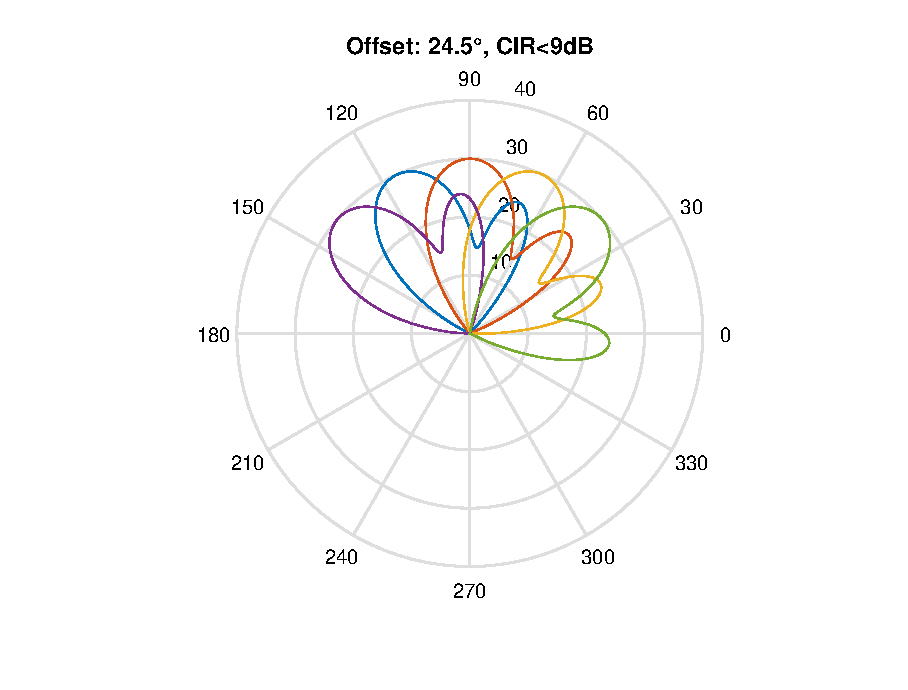
\includegraphics[width=11cm]{offset245deg.eps}
  \caption{Offset 24.5deg.}
  \label{fig:offset245deg}
\end{figure}

\begin{figure}[!h]
  \centering
  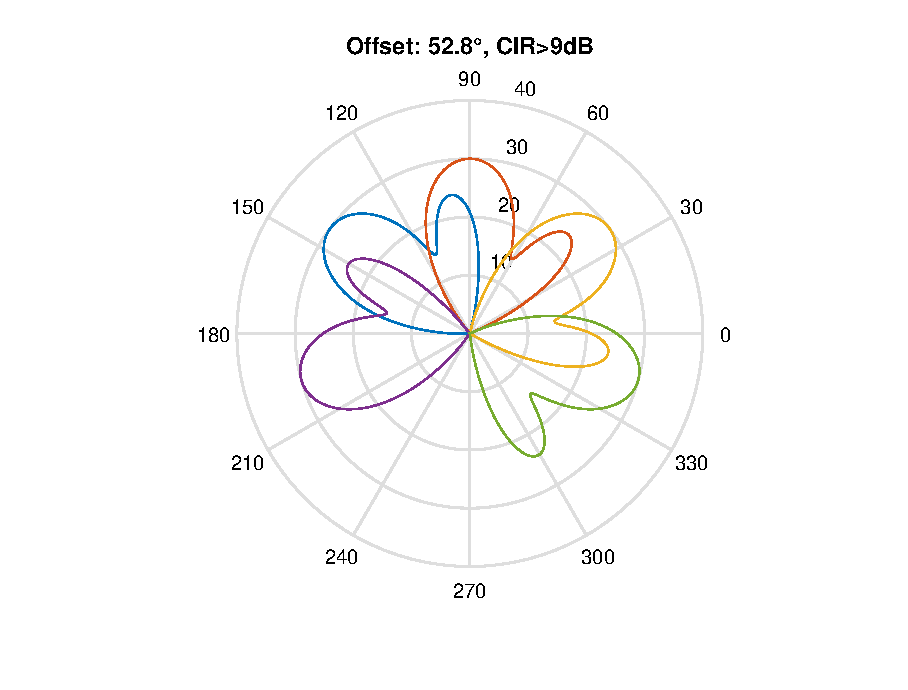
\includegraphics[width=11cm]{offset528deg.eps}
  \caption{Offset 52.8deg.}
  \label{fig:offset528deg}
\end{figure}

\begin{figure}[!h]
  \centering
  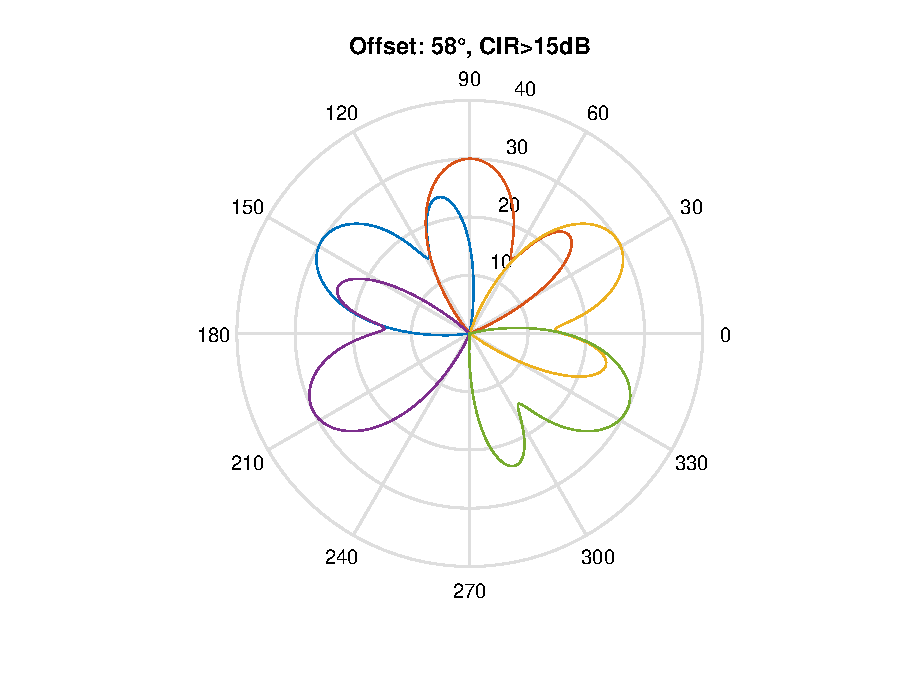
\includegraphics[width=11cm]{offset58deg.eps}
  \caption{Offset 58deg.}
  \label{fig:offset58deg}
\end{figure}

\begin{figure}[!h]
  \centering
  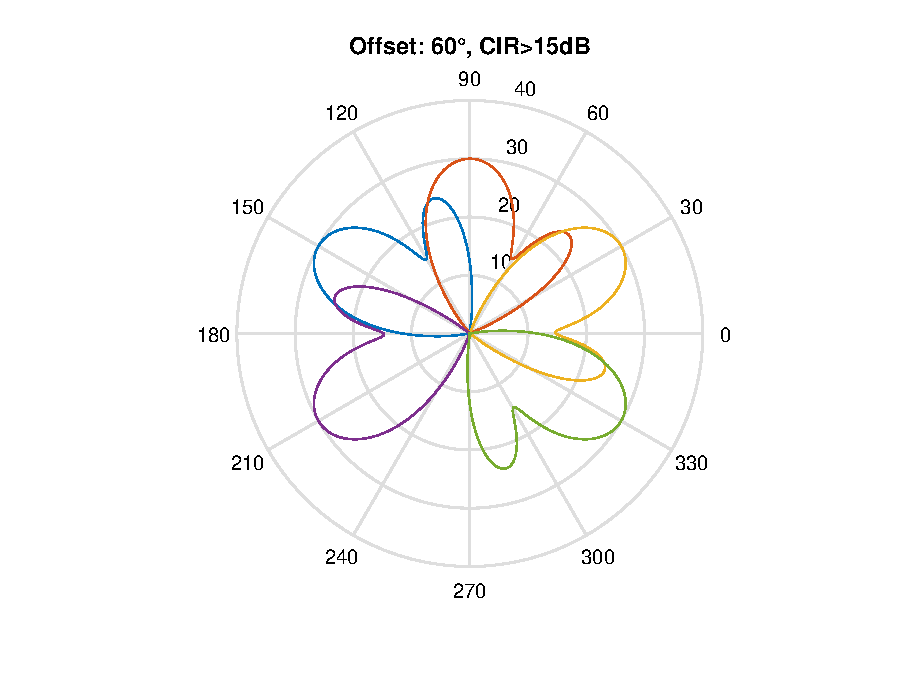
\includegraphics[width=11cm]{offset60deg.eps}
  \caption{Offset 60deg.}
  \label{fig:offset60deg}
\end{figure}

\subsubsection{b) How many spatially separated users can be served in the sector, under the conditions mentioned in a)?. I.e. what is N=?}


\subsection{Question 2}
\textit{Exchange the single path connections in exercise 1, to an angular uniform distribution over 20degree span and with a power density of 1 (similar to Cs in exercise A2). What changes result in the questions 1a) and 1b)?}

\section{Problem C}
\textit{REDUCING MAXIMUM PATH LOSS. For the same given coverage area, compare the maximum path loss of a single antenna system, $PL_{max^1}$, to the maximum path loss of an M-antenna distributed system, $PL_{max^M}$, and express the reduction in the dynamic range. Define path loss at the cell boundary, $d_c$, of the single-antenna system (as in the boxed expression above). State the implications of the relation.}\\

First the relation between the maximum path-loss for one and M antennas is described by \equref{eq:probc1} from problem B.\\

The maximum path-loss is form this exercise given by:
\begin{flalign}
&& PL_{max} \equiv & \frac{P_R}{P_{d_c}} = C\left(\frac{A_c}{\pi}\right)^{\sfrac{\gamma}{2}} & \label{eq:MaximumPathLoss}
\end{flalign}  

where $PL_{max}$ is the maximum pathloss, $P_R$ is the reference power which is equivalent to the transmitted power and $P_{d_c}$ is the minimum acceptable downlink power level at the cell boundary which is at the distance $d_c$ from the cell center (Radius of coverage area). $A_c$ is the coverage area of the cell and $\gamma$ is the pathloss exponent. C is a scaling constant. \\

From the hint given in the exercise we can derive the following:
\begin{flalign}
&& \frac{PL_{max}^M}{PL_{max}^1}  =& \frac{PL_{max}^1 \, M^{\frac{-\gamma}{2}}}{PL_{max}^1} = M^{\frac{-\gamma}{2}} & \label{eq:hintTBS} 
\end{flalign}
This relation between the two is however already shown in problem B.\\

This indicate that the higher the path-loss is the more advantages it is to use a distributed system.  


\section{Problem D}
\textit{Generate a few more channel realizations that follow the same power delay profile and let them be independent of the first set of channel realizations. Assume that these correspond to the channel impulse response from another transmit antenna.}
\section{Problem E}
\textit{Perform time reversal in a MISO context for each set of 2 channel realizations (one from A and one from D). Calculate the average power delay profile of the equivalent channel and from that the delay spread. How does it compare to the delay spread calculated in B and C? }

\chapter{MM2 - Spatial data multiplexing and space-time coding}
Advantages of using directive antennas -> space as 4th access/multiplex dimension\\

Beam space vs signal space methods (forward-reverse link sensitivity)\\

User tracking (link) vs traffic tracking (coverage)\\

Access vs interference suppression

\section{Exercise 1 - Problem 1}
\textit{ANALYTICAL: Select one of the code examples shown in class and show that they can achieve full diversity order.}\\

The code chosen was the one with three antennas and four symbols from the slides. This code however presented an error, so the used in this excersise was found in wikipedia, and it is the matrix $S$.\\

\begin{center}
$S=\begin{bmatrix}
s1 &-s2  &-s3  &-s4  &s1^{*}  &-s2^{*}  &-s3^{*}  &-s4^{*} \\ 
s2 &s1  &s4  &-s3  &s2^{*}  &s1^{*}  &s4^{*}  &-s3^{*} \\ 
s3 &-s4  &s1  &s2  &s3^{*}  &-s4^{*}  &s1^{*}  &s2^{*} 
\end{bmatrix}$\\
\end{center}

The first required step was to find the matrix E
\begin{flalign}
 && E =& S \cdot S^H & \label{eq:1_matrixE}
\end{flalign}

Once that matrix was found, the objective was to check if the rank was 3 (since there were 3 antennas); if this property was fulfilled, we could then say that the code achieved full diversity.\\

If the matrix E also resulted diagonal then this would mean that the evaluated code is also orthogonal.\\

The matrix E resulted to be (after correcting the error in the slide):\\

$\begin{bmatrix}
2 \left | s_{1} \right |^2 + 2 \left | s_{2} \right |^2 + 2 \left | s_{3} \right |^2 + 2 \left | s_{4} \right |^2& 0  & 0\\ 
 0& 2 \left | s_{1} \right |^2 + 2 \left | s_{2} \right |^2 + 2 \left | s_{3} \right |^2 + 2 \left | s_{4} \right |^2 &0 \\ 
 0&  0& 2 \left | s_{1} \right |^2 + 2 \left | s_{2} \right |^2 + 2 \left | s_{3} \right |^2 + 2 \left | s_{4} \right |^2
\end{bmatrix}$
\section{Exercise 1 - Problem 2}
\textit{MATLAB: Generate two channels that are independent, Rayleigh distributed and have equal average powers.}\\

This is done using the following code:
\code{language=Matlab,caption = Generation of Rayleigh distributed channels,label=cl:RayleighGeneration,linerange={5-23},firstnumber=5}{code/mm2/excercise2.m}

\FloatBarrier % Stops figs fucking arround
\subsection{a. Show the envelope distribution of the signals and the correlation coefficient.}
\fig[keepaspectratio=true,width=10cm]{ST_rayleigh_envelope_cor0.eps}{Envelope of uncorrelated Rayleigh fading channels}{fig:ST_rayleigh_envelope_cor0}
\fig[keepaspectratio=true,width=10cm]{ST_rayleigh_mrc_cor0.eps}{CDF of Rayleigh fading with MRC for uncorrelated channels}{fig:rayleigh_mrc_cor0}



\FloatBarrier % Stops figs fucking arround
\subsection{b. Implement the Alamouti scheme and find the resulting envelope distribution.}




\FloatBarrier % Stops figs fucking arround
\subsection{Repeat (a) and (b) for the case where the channels are correlated with $\rho=0.4$ }
To do this the same code is used as for question (a) but here the correlation is set to approximating $\rho=0.4$ this is giving the following plots:
\fig[keepaspectratio=true,width=10cm]{ST_rayleigh_envelope.eps}{Envelope of Rayleigh fading}{fig:ST_rayleigh_envelope}
\fig[keepaspectratio=true,width=10cm]{ST_rayleigh.eps}{CDF of Rayleigh fading}{fig:ST_rayleigh}
\fig[keepaspectratio=true,width=10cm]{ST_rayleigh_mrc.eps}{CDF of Rayleigh fading with MRC}{fig:ST_rayleigh_mrc}


\FloatBarrier % Stops figs fucking arround
\subsection{Repeat (a) and (b) for the case where the average power of the second channel is one half of the power of the first channel.}
\section{Exercise 2 - Problem 1}
\textit{From the expression of the MIMO channel capacity in terms of the normalized channel transfer matrix H \equref{eq:1_multiplexing}, derive the expression of the capacity in terms of the singular values l of H \equref{eq:2_multiplexing}.
Hint : remember how $H$ is decomposed - expand}
\begin{flalign}
 && C =& log_{2}\left(det\left(I + \frac{\rho}{M}HH^{H}\right) \right) & \label{eq:1_multiplexing}\\
\end{flalign}
The channel transfer matrix H can be expressed with the singular value decompression as 
\begin{flalign}
 && H =&  SUV^{H} &
\end{flalign}
where $S$ and $V$ are unitary matrices and $S$ the diagonal matrix containing the singular values of $H$. Inserting this into \equref{eq:1_multiplexing} the formula can be rearranged.
\begin{flalign}
 &&  C =& log_{2}\left(det\left(I + \frac{\rho}{M}SUV^{H}VU^{H}S^{H}\right) \right) & \\
 &&  =& log_{2}\left(det\left(I + \frac{\rho}{M}SUU^{H}S^{H}\right) \right) & 
 \end{flalign}
Expanding with $SS^{H}$
 \begin{flalign} 
 &&  C =& log_{2}\left(det\left[SS^{H}\left(I + \frac{\rho}{M}SUU^{H}S^{H}\right)SS^{H}\right] \right) & \\
 &&  =& log_{2}\left(det\left[S\left(I + \frac{\rho}{M}UU^{H}\right)S^{H}\right] \right) & \\
 &&  =& log_{2}\left(det\left(S\right)det\left(I + \frac{\rho}{M}UU^{H}\right)det\left(S^{H}\right) \right) & \\
 &&  =& log_{2}\left(det\left(SS^{H}\right)det\left(I + \frac{\rho}{M}UU^{H}\right) \right) & \\
 &&  =& log_{2}\left(det\left(I + \frac{\rho}{M}UU^{H}\right) \right) &
 \end{flalign}
 Where $U = diag(\lambda_i)$, with $\lambda_i=0$ for $i>rank(U)=rank(H)$
 
 \begin{flalign}
 &&  C =& log_{2}\left(det\left(I + \frac{\rho}{M}diag\left(\lambda^{2}_{i}\right)\right) \right) & \\
 &&  =& log_{2}\left(diag\left(1 + \frac{\rho}{M}\lambda^{2}_{i}\right)\right) & \\
 && =& log_{2}\left(\prod_{i = 1}^{k}\left(1 + \frac{\rho}{M}\lambda^{2}_{i}\right)\right) & \\
 && =& \sum_{i = 1}^{k}log_{2}\left(1 + \frac{\rho}{M}\lambda^{2}_{i}\right) & \label{eq:2_multiplexing}
\end{flalign}

\section{Exercise 2 - Problem 2}
\textit{To waterfill or not?}\\

\textit{Consider a 2x2 MIMO channel with ZMCSCG elements with unit variance. Develop your code for a square MIMO system of arbitrary number of antennas (and not just 2) since you will need it later in the problem. How does channel knowledge affect the Ergodic Capacity and the 10 percent Outage Capacity at low and high SNR values.} \\

\textit{Now increase the number of antennas to 4, 6 and 8 (remember the system is still MxM). How does channel knowledge affect ergodic capacity at 10 dB SNR with an increase in the number of antennas.}\\

ZMCSCG stands for Zero-Mean Circulant Symmetric Complex Gaussian. \\

The "water filling" principle implies assigning different values at the transmitted power for different transmit antennas according to channel performance, in order to increase capacity. This means that as it becomes better, the channel gets more power. \\

Using multiple transmit and receive antennas will help increase the capacity of the MIMO system. This can be seen from the capacity values obtained in Matlab, where the capacity formula is $C=C+log_{2}(1+SNR \lambda ^{2})$. The cdf plot for the obtained capacity values is shown in \figref{fig:MIMO_capacity} at 10 dB SNR.
\begin{figure}[!h]
  \centering
  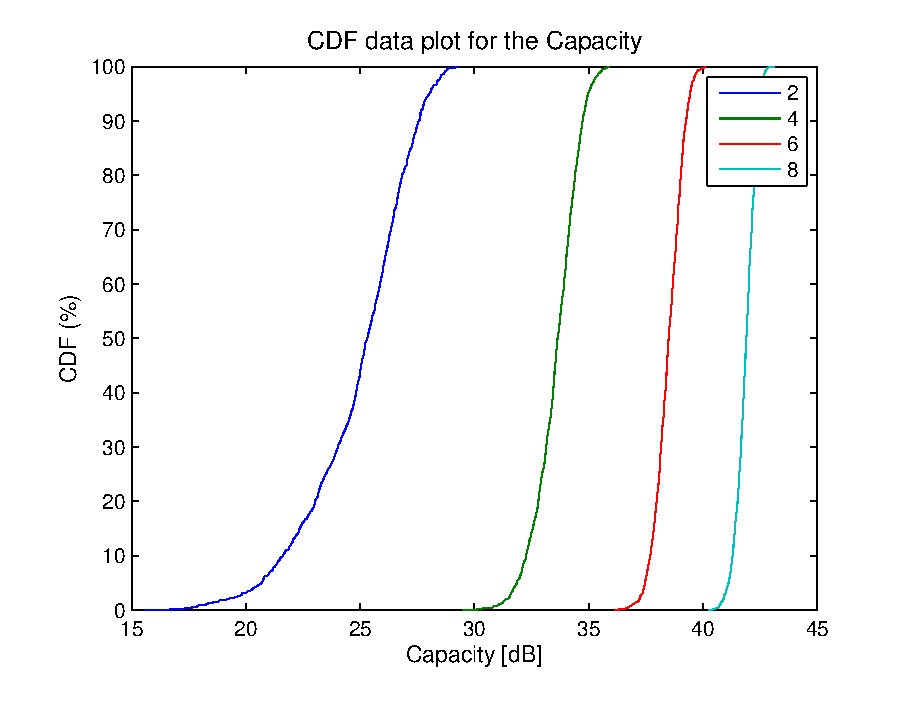
\includegraphics[width=10cm]{MIMO_capacity.eps}
  \caption{Capacity of a MIMO system using from 2 up to 8 antennas for 10dB SNR}
  \label{fig:MIMO_capacity}
\end{figure}
As it can be seen, using higher order MIMO implies an increase in capacity. By doubling the number of antennas from 2 to 4 and from 4 to 8, there is also an increase in capacity with 10 dB. \\

The capacity for low SNR values(1 dB) is shown in \figref{fig:MIMO_capacity_low_SNR}
\begin{figure}[!h]
  \centering
  \includegraphics[width=10cm]{MIMO_capacity_low_SNR.eps}
  \caption{Capacity of a MIMO system using from 2 up to 8 antennas for 1dB SNR}
  \label{fig:MIMO_capacity_low_SNR}
\end{figure}
%The channel capacity is also higly related to the correlation between transmit and receive antennas. The capacity is reduced as the correlation becomes higher.
%The maximum outage capacity can be defined as the maximum rate that can be maintained in all channel states with some probability of outage (no data transmission).


\part{Troels Part 1}
\chapter{MM3 - Distributed antenna systems}
Advantages of using directive antennas -> space as 4th access/multiplex dimension\\

Beam space vs signal space methods (forward-reverse link sensitivity)\\

User tracking (link) vs traffic tracking (coverage)\\

Access vs interference suppression

\section{Problem A} \label{sec:mm3_PbA}
\textit{MAXIMISING COVERAGE AREA. For a given radiated power, compare the coverage area of a single antenna system, $Ac^1$, to the coverage area of an M-antenna distributed antenna system, $Ac^M$. State the implications of the relation.}\\

We assume, that the minimum acceptable downlink power remains the same for both the single antenna system and the M-antenna system. Also, the total radiated power is constant, so it is divided onto the M antennas. The addition of an index M denotes the belonging to the M-antenna system, so for example $A_c$ is the coverage area of the single antenna system, while $A_{cM}$ is the M-antenna system cell coverage area. 

\begin{flalign}
&& P_{dc} &= P_{dc,M} &\\
&& &=const. &\\
&&\frac{PL}{P_R} &=M \cdot \frac{PL_M}{P_R} &\\
&& PL&=M\cdot PL_M & \label{eq:pathloss_1_M}
\end{flalign}

The relationship between the path loss and the coverage area is given as

\begin{flalign}
PL = C \left(\frac{A_c}{\pi}\right)^\frac{\gamma}{2}. 
\end{flalign}

This can be inserted to \eqref{eq:pathloss_1_M} to find the relation between the coverage area in both cases.

\begin{flalign}
\left(\frac{A_c}{\pi}\right)^{\frac{\gamma}{2}}=M\cdot\left(\frac{A_{cM}}{\pi}\right)^{\frac{\gamma}{2}}\\
A_c^{\frac{\gamma}{2}}=M\cdot (A_{cM})^{\frac{\gamma}{2}}\\
A_c=M^{\frac{2}{\gamma}}\cdot A_{cM} \\
\frac{A_{cM}}{A_{c}} =M^{-\frac{2}{\gamma}} \label{eq:ExpressionForAcWithM} \\
\frac{A_{cM,total}}{A_{c}} =\frac{A_{cM}\cdot M}{A_{c}}=M^{-\frac{2}{\gamma}+1}
\end{flalign}

The implications of this factor are shown in \figref{fig:Acm_M}, \figref{fig:Acmtot_M}, \figref{fig:Acm_gamma}, \figref{fig:Acmtot_gamma} and \figref{fig:Acmtot_gamma_M}. [Additional text to describe implications...?]

\fig[keepaspectratio=true,width=11cm]{Acm_M.eps}{Coverage Area of one cell for multiple antennas vs. antenna number.}{fig:Acm_M}

\fig[keepaspectratio=true,width=11cm]{Acmtot_M.eps}{Total coverage Area for multiple antennas vs. antenna number.}{fig:Acmtot_M}

\fig[keepaspectratio=true,width=11cm]{Acm_gamma.eps}{Coverage Area of one cell for multiple antennas vs. PL coefficient.}{fig:Acm_gamma}

\fig[keepaspectratio=true,width=11cm]{Acmtot_gamma.eps}{Total coverage Area for multiple antennas vs. PL coefficient.}{fig:Acmtot_gamma}

\fig[keepaspectratio=true,width=11cm]{Acmtot_gamma_M.eps}{Total coverage Area vs. PL coefficient and number of antennas.}{fig:Acmtot_gamma_M}



\section{Problem B - SDMA aspect}
\textit{Use the defined antenna patterns/directional signals from exercise A . You would need also some results/idea about exercise A2, if not finished (remember two main tasks : one to find C/I with directional spread signals, other to find shape of full radar sweep (effective antenna pattern wrt user and interferer) and resulting mean direction)}

\subsection{Question 1}
\textit{Now consider a 120 degree sector serviced with above antenna pattern in a SDMA operation (i.e. identical but offset patterns for N users). Consider the system to have power control so all users have same power received at the BS when the individual users antenna pattern maximum is pointed to their respective direction. Assume only a single path from user to BS (like exercise A1))}

\subsubsection{a) For a target C/I=9dB (spatial interference), what is the required user-to-interferer offset angle (to left and right)?. If C/I is 15 dB what then?}

\begin{figure}[!h]
  \centering
  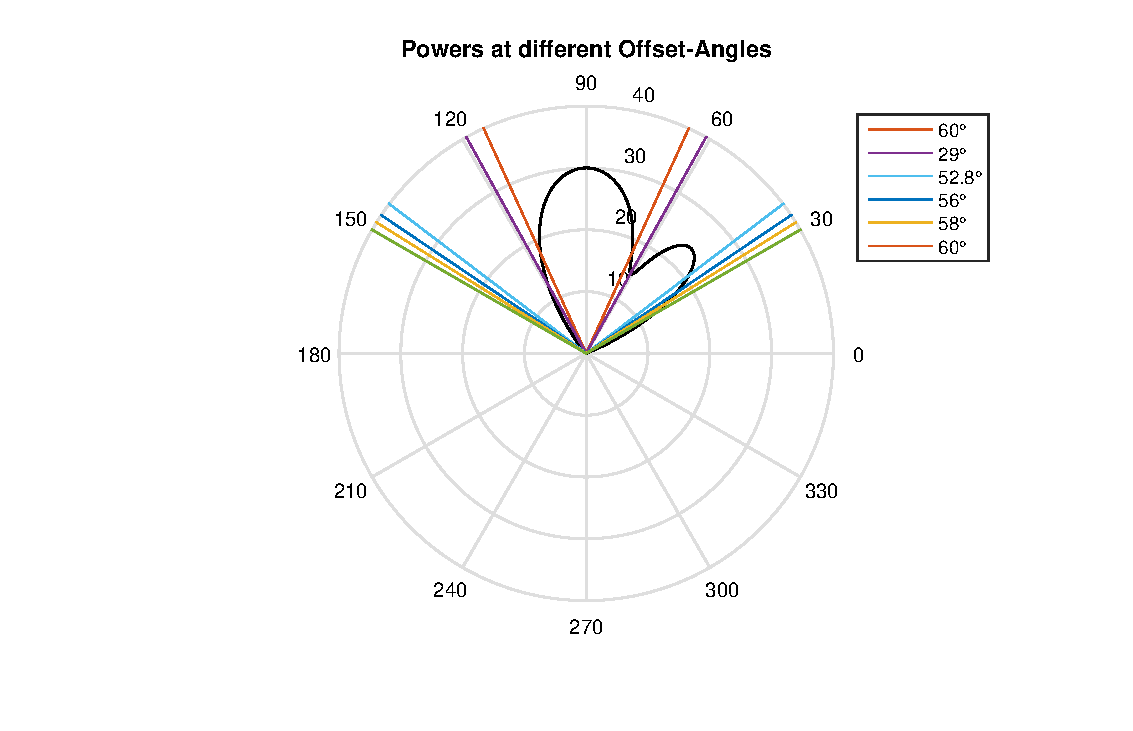
\includegraphics[width=12cm]{offset_angles.eps}
  \caption{Offset angles.}
  \label{fig:offset_angles}
\end{figure}

\begin{figure}[!h]
  \centering
  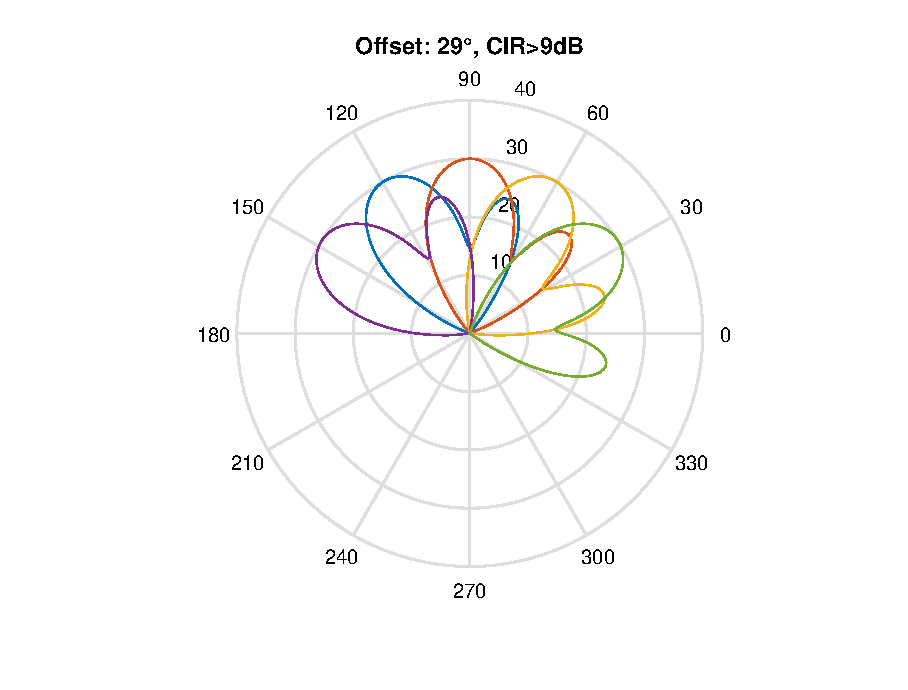
\includegraphics[width=11cm]{offset29deg.eps}
  \caption{Offset 29deg.}
  \label{fig:offset29deg}
\end{figure}

\begin{figure}[!h]
  \centering
  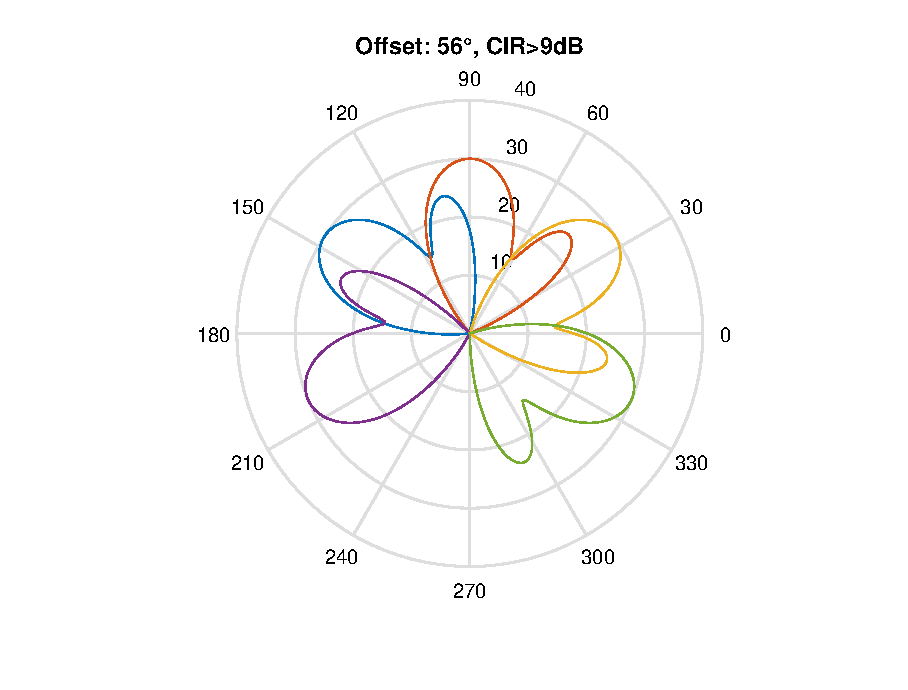
\includegraphics[width=11cm]{offset56deg.eps}
  \caption{Offset 56deg.}
  \label{fig:offset56deg}
\end{figure}

\begin{figure}[!h]
  \centering
  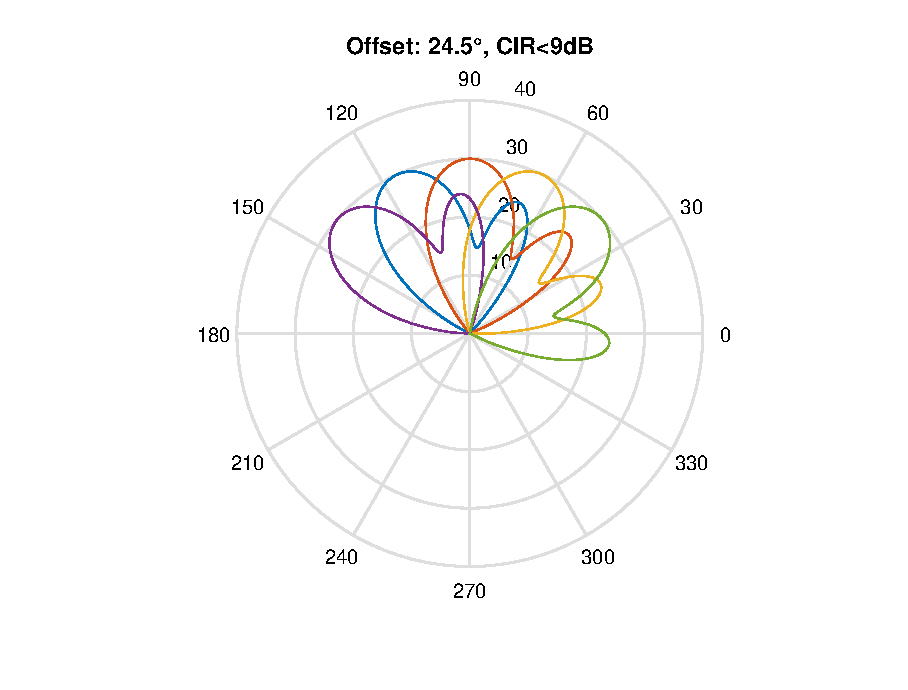
\includegraphics[width=11cm]{offset245deg.eps}
  \caption{Offset 24.5deg.}
  \label{fig:offset245deg}
\end{figure}

\begin{figure}[!h]
  \centering
  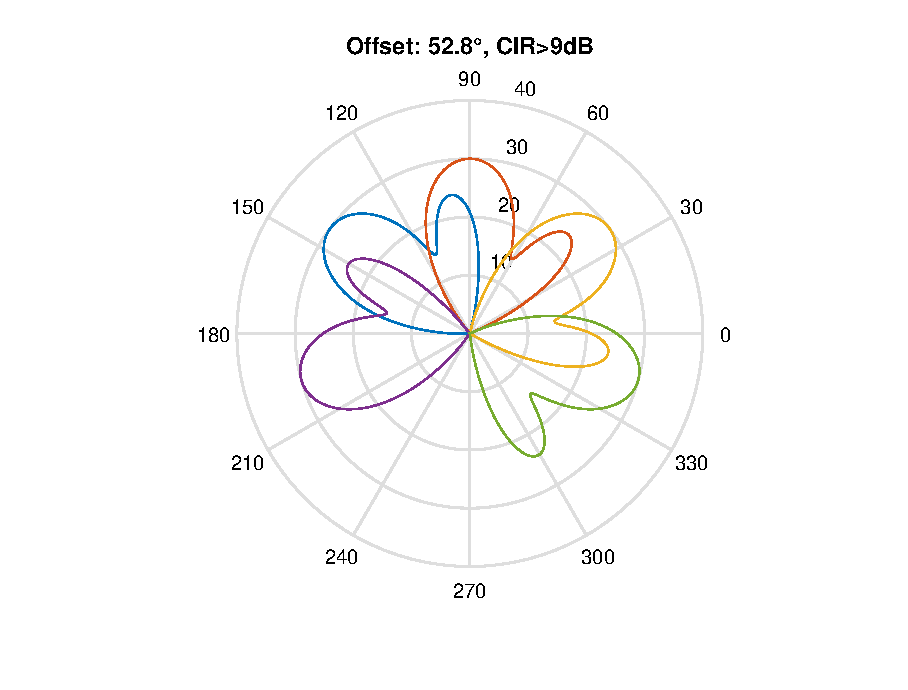
\includegraphics[width=11cm]{offset528deg.eps}
  \caption{Offset 52.8deg.}
  \label{fig:offset528deg}
\end{figure}

\begin{figure}[!h]
  \centering
  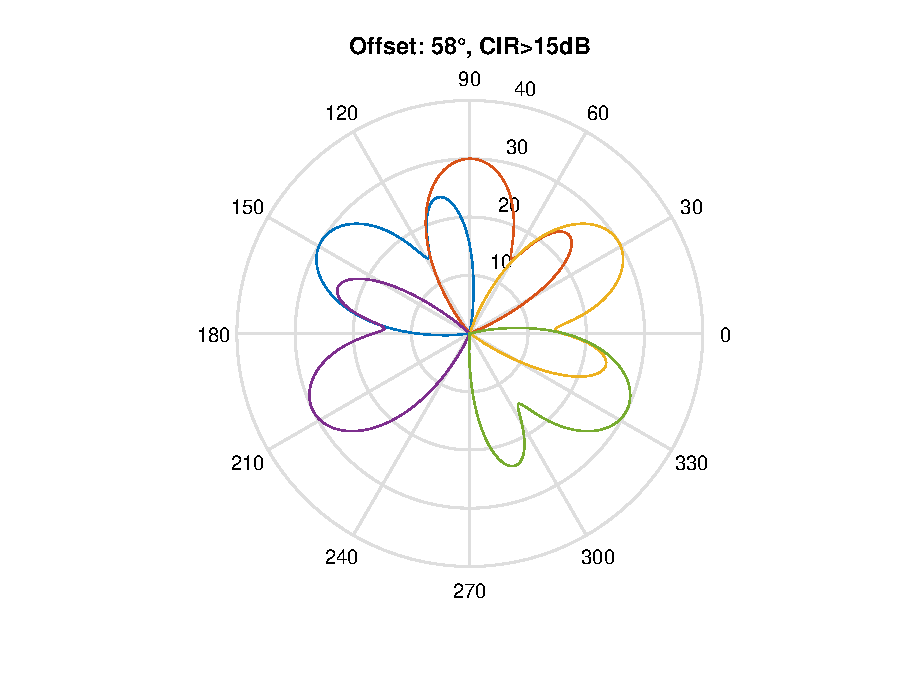
\includegraphics[width=11cm]{offset58deg.eps}
  \caption{Offset 58deg.}
  \label{fig:offset58deg}
\end{figure}

\begin{figure}[!h]
  \centering
  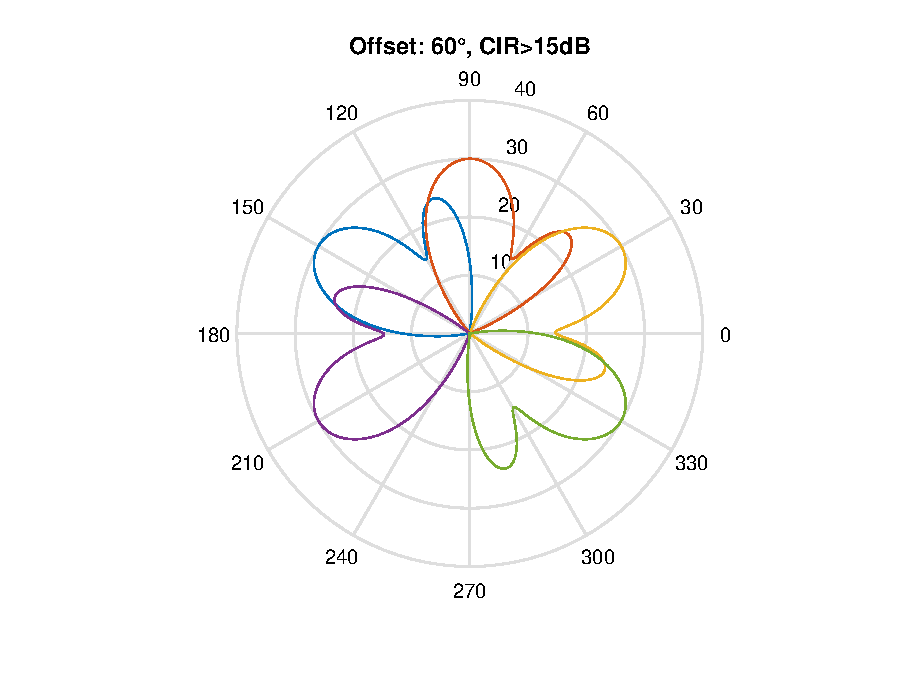
\includegraphics[width=11cm]{offset60deg.eps}
  \caption{Offset 60deg.}
  \label{fig:offset60deg}
\end{figure}

\subsubsection{b) How many spatially separated users can be served in the sector, under the conditions mentioned in a)?. I.e. what is N=?}


\subsection{Question 2}
\textit{Exchange the single path connections in exercise 1, to an angular uniform distribution over 20degree span and with a power density of 1 (similar to Cs in exercise A2). What changes result in the questions 1a) and 1b)?}

\section{Problem C}
\textit{REDUCING MAXIMUM PATH LOSS. For the same given coverage area, compare the maximum path loss of a single antenna system, $PL_{max^1}$, to the maximum path loss of an M-antenna distributed system, $PL_{max^M}$, and express the reduction in the dynamic range. Define path loss at the cell boundary, $d_c$, of the single-antenna system (as in the boxed expression above). State the implications of the relation.}\\

First the relation between the maximum path-loss for one and M antennas is described by \equref{eq:probc1} from problem B.\\

The maximum path-loss is form this exercise given by:
\begin{flalign}
&& PL_{max} \equiv & \frac{P_R}{P_{d_c}} = C\left(\frac{A_c}{\pi}\right)^{\sfrac{\gamma}{2}} & \label{eq:MaximumPathLoss}
\end{flalign}  

where $PL_{max}$ is the maximum pathloss, $P_R$ is the reference power which is equivalent to the transmitted power and $P_{d_c}$ is the minimum acceptable downlink power level at the cell boundary which is at the distance $d_c$ from the cell center (Radius of coverage area). $A_c$ is the coverage area of the cell and $\gamma$ is the pathloss exponent. C is a scaling constant. \\

From the hint given in the exercise we can derive the following:
\begin{flalign}
&& \frac{PL_{max}^M}{PL_{max}^1}  =& \frac{PL_{max}^1 \, M^{\frac{-\gamma}{2}}}{PL_{max}^1} = M^{\frac{-\gamma}{2}} & \label{eq:hintTBS} 
\end{flalign}
This relation between the two is however already shown in problem B.\\

This indicate that the higher the path-loss is the more advantages it is to use a distributed system.  


\section{Problem D}
\textit{Generate a few more channel realizations that follow the same power delay profile and let them be independent of the first set of channel realizations. Assume that these correspond to the channel impulse response from another transmit antenna.}

\part{Patrick Part 2}
\chapter{MM4 - Advantages of using directive antennas (SDMA)}
Advantages of using directive antennas -> space as 4th access/multiplex dimension\\

Beam space vs signal space methods (forward-reverse link sensitivity)\\

User tracking (link) vs traffic tracking (coverage)\\

Access vs interference suppression

\section{Problem A} \label{sec:mm3_PbA}
\textit{MAXIMISING COVERAGE AREA. For a given radiated power, compare the coverage area of a single antenna system, $Ac^1$, to the coverage area of an M-antenna distributed antenna system, $Ac^M$. State the implications of the relation.}\\

We assume, that the minimum acceptable downlink power remains the same for both the single antenna system and the M-antenna system. Also, the total radiated power is constant, so it is divided onto the M antennas. The addition of an index M denotes the belonging to the M-antenna system, so for example $A_c$ is the coverage area of the single antenna system, while $A_{cM}$ is the M-antenna system cell coverage area. 

\begin{flalign}
&& P_{dc} &= P_{dc,M} &\\
&& &=const. &\\
&&\frac{PL}{P_R} &=M \cdot \frac{PL_M}{P_R} &\\
&& PL&=M\cdot PL_M & \label{eq:pathloss_1_M}
\end{flalign}

The relationship between the path loss and the coverage area is given as

\begin{flalign}
PL = C \left(\frac{A_c}{\pi}\right)^\frac{\gamma}{2}. 
\end{flalign}

This can be inserted to \eqref{eq:pathloss_1_M} to find the relation between the coverage area in both cases.

\begin{flalign}
\left(\frac{A_c}{\pi}\right)^{\frac{\gamma}{2}}=M\cdot\left(\frac{A_{cM}}{\pi}\right)^{\frac{\gamma}{2}}\\
A_c^{\frac{\gamma}{2}}=M\cdot (A_{cM})^{\frac{\gamma}{2}}\\
A_c=M^{\frac{2}{\gamma}}\cdot A_{cM} \\
\frac{A_{cM}}{A_{c}} =M^{-\frac{2}{\gamma}} \label{eq:ExpressionForAcWithM} \\
\frac{A_{cM,total}}{A_{c}} =\frac{A_{cM}\cdot M}{A_{c}}=M^{-\frac{2}{\gamma}+1}
\end{flalign}

The implications of this factor are shown in \figref{fig:Acm_M}, \figref{fig:Acmtot_M}, \figref{fig:Acm_gamma}, \figref{fig:Acmtot_gamma} and \figref{fig:Acmtot_gamma_M}. [Additional text to describe implications...?]

\fig[keepaspectratio=true,width=11cm]{Acm_M.eps}{Coverage Area of one cell for multiple antennas vs. antenna number.}{fig:Acm_M}

\fig[keepaspectratio=true,width=11cm]{Acmtot_M.eps}{Total coverage Area for multiple antennas vs. antenna number.}{fig:Acmtot_M}

\fig[keepaspectratio=true,width=11cm]{Acm_gamma.eps}{Coverage Area of one cell for multiple antennas vs. PL coefficient.}{fig:Acm_gamma}

\fig[keepaspectratio=true,width=11cm]{Acmtot_gamma.eps}{Total coverage Area for multiple antennas vs. PL coefficient.}{fig:Acmtot_gamma}

\fig[keepaspectratio=true,width=11cm]{Acmtot_gamma_M.eps}{Total coverage Area vs. PL coefficient and number of antennas.}{fig:Acmtot_gamma_M}



\subsection{Question 2}
\textit{The user and interferer are now replaced by angular distribution of: Cs($\Phi$)= 1 within 80 to 100 deg. , 0 outside and Is($\Phi$)=3/4 within 54 to 67 deg., 0 outside}

\subsubsection{a) what is the peak to null depth for the measured response of the user compared to max and sidelobe}

To answer this question we need to find the azimuthal measurement response. This is done finding the correlation function between the environment as a function of $\varphi$, and the antenna pattern as shown in \equref{eq:effective}.

\begin{flalign}
&&	m(\varphi) =& \oint e(\Phi) \cdot a(\Phi - \varphi)d\Phi =R_{e,a^{*}}(\varphi)	 &\label{eq:effective}
\end{flalign}

The resulting pattern is shown in \textbf{FIGURE}. From which, graphically, the peak to null depth can be calculated  \textbf{PUT THE CALCULATED RESULT}

\subsubsection{b) What is the Cs/Is of the measured responses and what direction will the response function be centered at if performing a sweep (radar scan) with the antenna on the user and on the interferer?}

This value can be computed by two different methods. One is to integrate the product of the antenna pattern and the angular distribution of the users over the whole circle as shown in \equref{eq:bruteforce}.

\begin{flalign}
&&	\frac{Cs}{Is} =& \frac{\oint C(\varphi)\cdot a(\varphi)d\varphi}{\oint I(\varphi)\cdot a(\varphi)d\varphi}	 &\label{eq:bruteforce}
\end{flalign}

Another method to compute this result is to use the azimuthal measurement response of both, the user and the interferer. In the previous question, the graph of the $m_{C}(\varphi)$ was shown and in figure INSERT FIGURE $m_{I}(\varphi)$ we show this response for the interferer in \textbf{FIGURE}.

Mathematically, performing a sweep (radar scan) is equivalent to find the correlation function described in \equref{eq:effective}. Due to the properties of this ``convolution'', the user (whose mean is located at 90 degrees) will be shifted $90 + 90$ degrees. As seen in \textbf{FIGURE}. The interferer, because of the same argument, will be shifted $60.5 + 60.5$ degrees.

In order to compute this result by this second method, we need to calculate the $Cs$ and the $Is$ using $m_{C}(\varphi)$ and $m_{I}(\varphi)$. This is done considering the user as a single source in $m_{C}(\varphi)$ at 180 degrees and the interferer as a single source in $m_{I}(\varphi)$ at 121 degrees. \textbf{MAYBE EXPAND THIS EXPLANATION}
\section{Problem B - SDMA aspect}
\textit{Use the defined antenna patterns/directional signals from exercise A . You would need also some results/idea about exercise A2, if not finished (remember two main tasks : one to find C/I with directional spread signals, other to find shape of full radar sweep (effective antenna pattern wrt user and interferer) and resulting mean direction)}

\subsection{Question 1}
\textit{Now consider a 120 degree sector serviced with above antenna pattern in a SDMA operation (i.e. identical but offset patterns for N users). Consider the system to have power control so all users have same power received at the BS when the individual users antenna pattern maximum is pointed to their respective direction. Assume only a single path from user to BS (like exercise A1))}

\subsubsection{a) For a target C/I=9dB (spatial interference), what is the required user-to-interferer offset angle (to left and right)?. If C/I is 15 dB what then?}

\begin{figure}[!h]
  \centering
  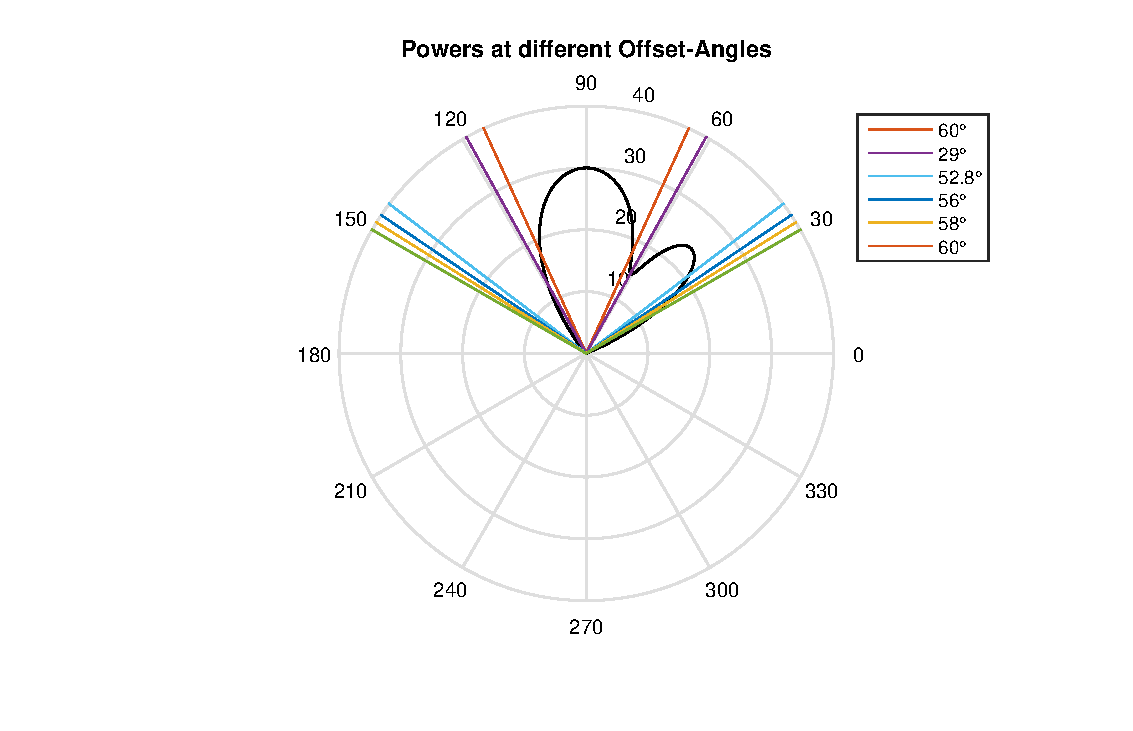
\includegraphics[width=12cm]{offset_angles.eps}
  \caption{Offset angles.}
  \label{fig:offset_angles}
\end{figure}

\begin{figure}[!h]
  \centering
  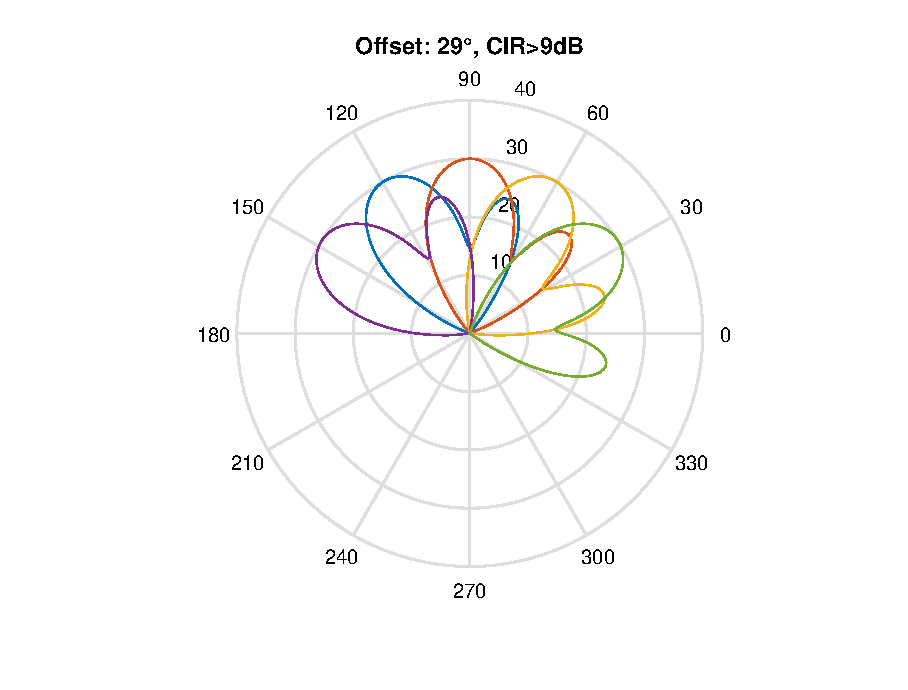
\includegraphics[width=11cm]{offset29deg.eps}
  \caption{Offset 29deg.}
  \label{fig:offset29deg}
\end{figure}

\begin{figure}[!h]
  \centering
  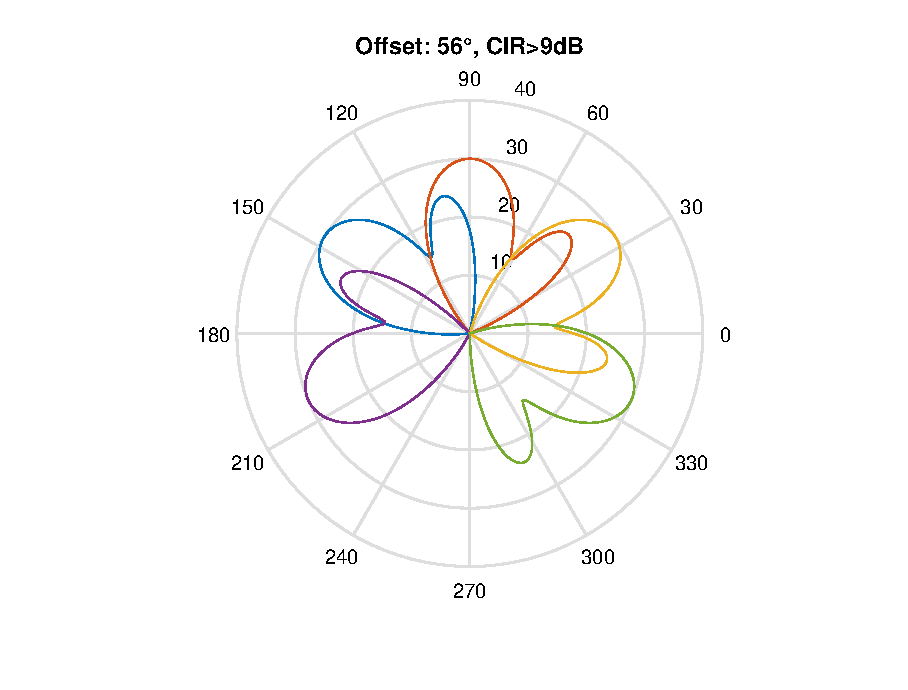
\includegraphics[width=11cm]{offset56deg.eps}
  \caption{Offset 56deg.}
  \label{fig:offset56deg}
\end{figure}

\begin{figure}[!h]
  \centering
  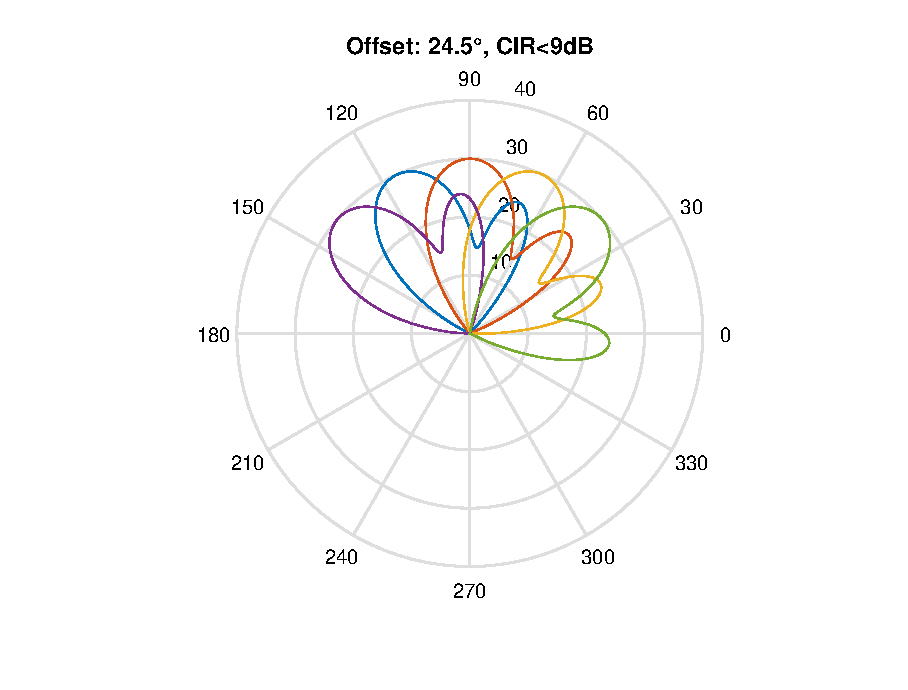
\includegraphics[width=11cm]{offset245deg.eps}
  \caption{Offset 24.5deg.}
  \label{fig:offset245deg}
\end{figure}

\begin{figure}[!h]
  \centering
  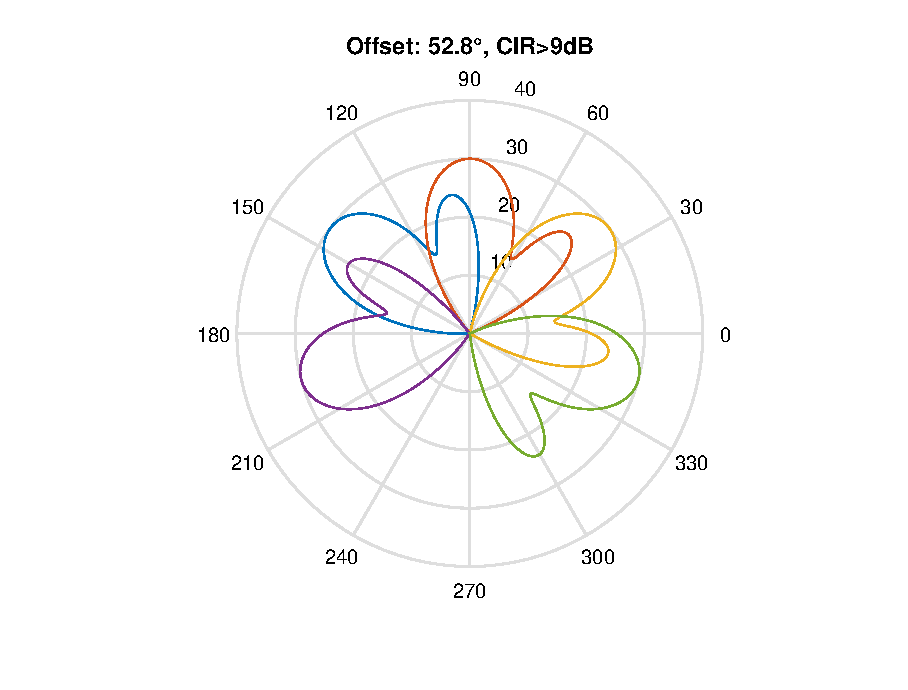
\includegraphics[width=11cm]{offset528deg.eps}
  \caption{Offset 52.8deg.}
  \label{fig:offset528deg}
\end{figure}

\begin{figure}[!h]
  \centering
  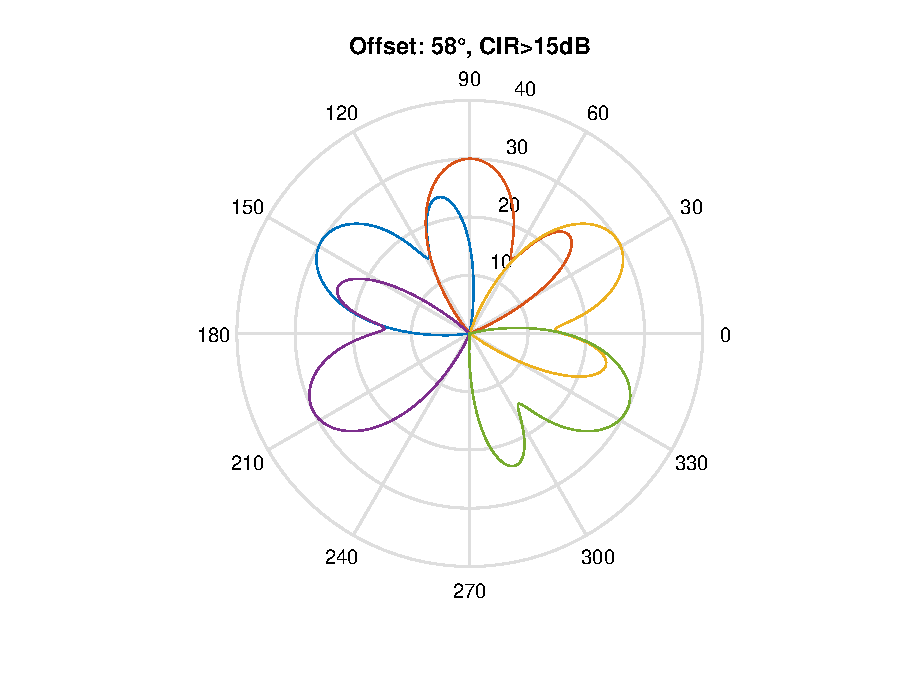
\includegraphics[width=11cm]{offset58deg.eps}
  \caption{Offset 58deg.}
  \label{fig:offset58deg}
\end{figure}

\begin{figure}[!h]
  \centering
  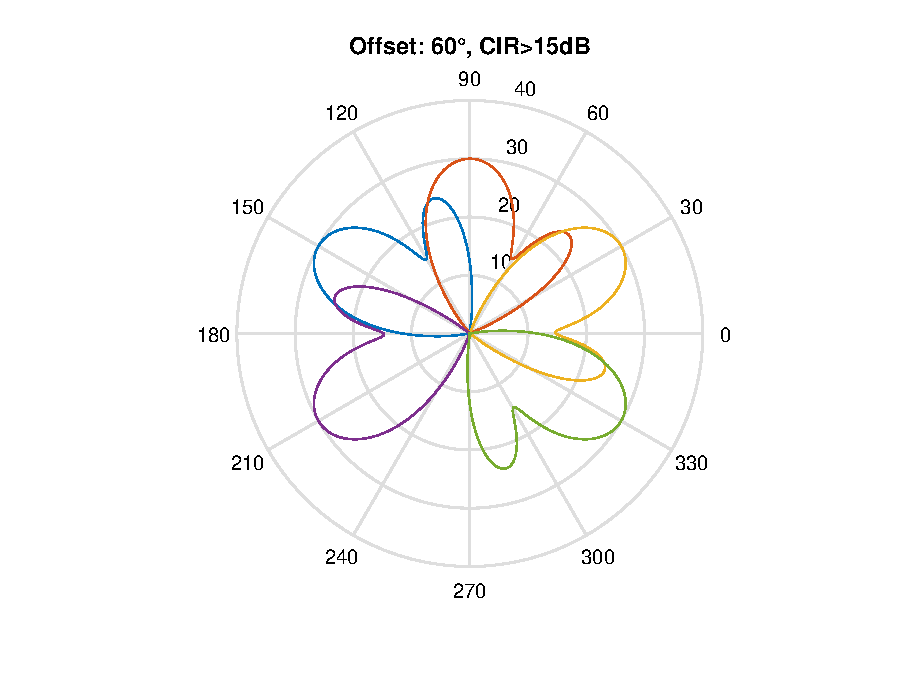
\includegraphics[width=11cm]{offset60deg.eps}
  \caption{Offset 60deg.}
  \label{fig:offset60deg}
\end{figure}

\subsubsection{b) How many spatially separated users can be served in the sector, under the conditions mentioned in a)?. I.e. what is N=?}


\subsection{Question 2}
\textit{Exchange the single path connections in exercise 1, to an angular uniform distribution over 20degree span and with a power density of 1 (similar to Cs in exercise A2). What changes result in the questions 1a) and 1b)?}


\part{Petar - Multi-user Communication over a Shared Medium}
\chapter{MM5 - Cross-layer optimized design of wireless systems}
Advantages of using directive antennas -> space as 4th access/multiplex dimension\\

Beam space vs signal space methods (forward-reverse link sensitivity)\\

User tracking (link) vs traffic tracking (coverage)\\

Access vs interference suppression

\section{Problem 1}
\textit{Prove using the equivalence theorem that an electric current source does not radiate when it 
is tangential to a perfect electric conductor.}\\

Greens Function and the vector potential functions can only be used in free space or a homogeneous medium. Since we now have to deal with a electric current source tangential to a perfect electric conductor, we cannot directly compute the fields with the above procedure. First we have to transform the problem to a free space problem. This can be done using the surface equivalence theorem, which yields an equivalent image or mirror source of the incident electric current as a replacement of the PEC wall as can be seen from \figref{fig:imagetheory}. 

\begin{figure}[!h]
  \centering
  


\psscalebox{1.0 1.0} % Change this value to rescale the drawing.
{
\begin{pspicture}(0,-2.4200153)(4.18,2.4200153)
\psline[linecolor=black, linewidth=0.04](0.72,2.4000154)(0.72,-2.3999848)(0.72,-2.3999848)(0.72,-2.3999848)(0.72,-1.9999847)
\psline[linecolor=black, linewidth=0.04, arrowsize=0.05291666666666667cm 2.0,arrowlength=1.4,arrowinset=0.0]{->}(0.32,-0.79998475)(0.32,0.8000153)
\rput[bl](0.0,0.10001526){J}
\psframe[linecolor=white, linewidth=0.04, fillstyle=vlines*, hatchwidth=0.028222222, hatchangle=45.0, hatchsep=0.1411111, dimen=outer](1.12,2.4000154)(0.72,-2.3999848)
\psline[linecolor=black, linewidth=0.04, linestyle=dotted, dotsep=0.10583334cm](3.52,2.4000154)(3.52,-2.3999848)(3.52,-2.3999848)(3.52,-2.3999848)(3.52,-1.9999847)
\psline[linecolor=black, linewidth=0.04, arrowsize=0.05291666666666667cm 2.0,arrowlength=1.4,arrowinset=0.0]{->}(3.12,-0.79998475)(3.12,0.8000153)
\rput[bl](2.8,0.10001526){J}
\rput[bl](1.12,-1.9999847){PEC}
\psline[linecolor=black, linewidth=0.04, arrowsize=0.05291666666666667cm 2.0,arrowlength=1.4,arrowinset=0.0]{<-}(3.92,-0.79998475)(3.92,0.8000153)
\rput[bl](4.0,0.10001526){J}
\end{pspicture}
}
  \caption{Equivalent model for electric source near a perfect electric conductor (PEC).}
  \label{fig:imagetheory}
\end{figure}

Since the image source which replaces the PEC wall is located in the same distance from the PEC boundary as the actual source but with reversed orientation we now can calculate the resulting fields as a superposition of the fields from the two sources in free space. Since the real source is located tangential to the PEC wall with a negligible distance from it, the two sources can be seen as in the same point and can be summarized to one source, which then of course is zero. From this we can easily conclude, that the electric current source tangential to a perfect electric conductor does not radiate. 




\section{Problem 2}
\textit{a) Find the MEG for a vertically mounted half wave dipole, $Gain(\theta, \Phi) = 1.5 \cdot \sin(\theta)$, for an 
environment where all power is coming from the azimuthal plane (xy-plane) and in theta polarization only.}

For a vertically mounted half wave dipole, we can assume, that the $XPR$ (cross polarization power ratio) is infinite. In addition, we can make the following assumptions for the $\phi$ and $\theta$ components of the angular density functions of the incoming waves

\begin{flalign}
&& P_\phi &= 0 &\\
&& P_\theta &= \frac{ \delta(\theta-\SI{90}{\degree}) }{sin(\SI{90}{\degree})} &\\
&& &= \delta(\theta-\SI{90}{\degree}) &
\end{flalign}

with the Delta-Dirac-Distribution $\delta$. Using this, we can calculate the MEG.

\begin{flalign}
&& G_e &= \int_0^{2\pi}  \! \int_0^\pi  \! \frac{XPR}{1+XPR} G_\theta P_\theta \sin{\theta} \, \mathrm{d}\theta \, \mathrm{d}\phi &\\
&& &= \int_0^{2\pi}  \! \int_0^\pi 1.5  \! \sin^2{\theta} \delta(\theta-\SI{90}{\degree})  \, \mathrm{d}\theta \, \mathrm{d}\phi &\\
&& &= 2\pi \int_0^\pi  \! 1.5 \sin^2{\theta} \delta(\theta-\SI{90}{\degree})  \, \mathrm{d}\theta &\\
&& &= 3\pi \cdot \sin^2(\SI{90}{\degree}) &\\
&& &= 3\pi. &
\end{flalign}

\textit{b) Now, the dipole is rotated 90 degrees (along the X axis), what is the MEG?}

Since now due to the horizontally aligned half wave dipole, we can assume $XPR=0$. This way, the integrand reduces to zero, so

\begin{flalign}
G_e=   0.
\end{flalign}
\section{Problem 3} \label{sec:mm5_Pb3}
\textit{A terminal is applying the slotted ALOHA protocol in the following way:
\begin{description}
 \item [Step 1] If the terminal has a new packet for transmission, it immediately transmits it (i. e. at the next start of a new slot)
 \item [Step 2] If the packet is in error, then the terminal 
 \begin{itemize}
  \item Transmits the packet with probability q in the next slot
  \item Is quiet during the next slot with probability (1-q)
 \end{itemize}
 \item [Step 3] Repeats Step 2 until the packet is transmitted correctly
 \item [Step 4] Gets a new packet
 \end{description}
Assume that the probability of packet error due to the noise is $P_{e}$. Assume that each packet has D bits and the packet duration is equal to the slot durations T. There is only one terminal in the system which communicates with a Base station, such that there are no collisions in the system and a packet can be lost only due to the noise. A new packet arrives to terminal whenever the previous packet has been transmitted correctly.}
\subsection {a)}
\textit{What is the maximal throughput that the terminal can achieve?}
The terminal transmit the packet with an error of $P_{e}$ and retransmit it with probability q. The probability that the retransmitting is failing is the probability that it retransmit multiplied with the probability of fail. $P(retransmit|fail) = P_{e} \cdot q$ So the probability that the terminal successfully transmit the packet is $P(succes) = 1 - q\cdot P_{e}$. 

The maximum throughput is then given by
\begin{flalign}
 G_{aloha} = P(success) \cdot \frac{D}{T}
\end{flalign}

\subsection {b)}
\textit{What is the throughput that the terminal can achieve if it turns off the ALOHA protocol and retransmits the packet until successful transmission?} 
If it transmit right away q is set equal 1. 
\begin{flalign}
 && G_{noAloha} = & (1-P_{e})\frac{D}{T_{s}} &
\end{flalign}

\section{Problem 4}
\textit{Alfa equal 55 degrees is claimed to be a good references – why? B) and why then measure in both 0, 90, 45 and -45 degrees and not 55 degrees?}

To make an evaluation of the environment it is needed to minimize the effect produced by the different polarizations in the received waves in such area. To reduce this effect it can be proved that for a half-length dipole, the mean effective gain (MEG) is the same independently of the cross polarization ratio $XPR$, when said dipole is inclined 55 degrees in its elevation angle.

When said dipole is inclined, it defines a plane (called antenna inclination plane in the bibliography). Subsequently, to evaluate the environment in which the antenna is located, this antenna inclination plane is then rotated in $\Phi$ (the azimuth angle) and the power measurements are performed.

In figure \figref{fig:dipole_inclination} it can be seen the angle $\alpha$ (which is set to 55 degrees in the experiment) and the angle $\Phi$ in which the antenna inclination angle is rotated. It can be mention that in the figure, the vector $L$ is in the antenna inclination plane.


\begin{figure}[!h]
  \centering
  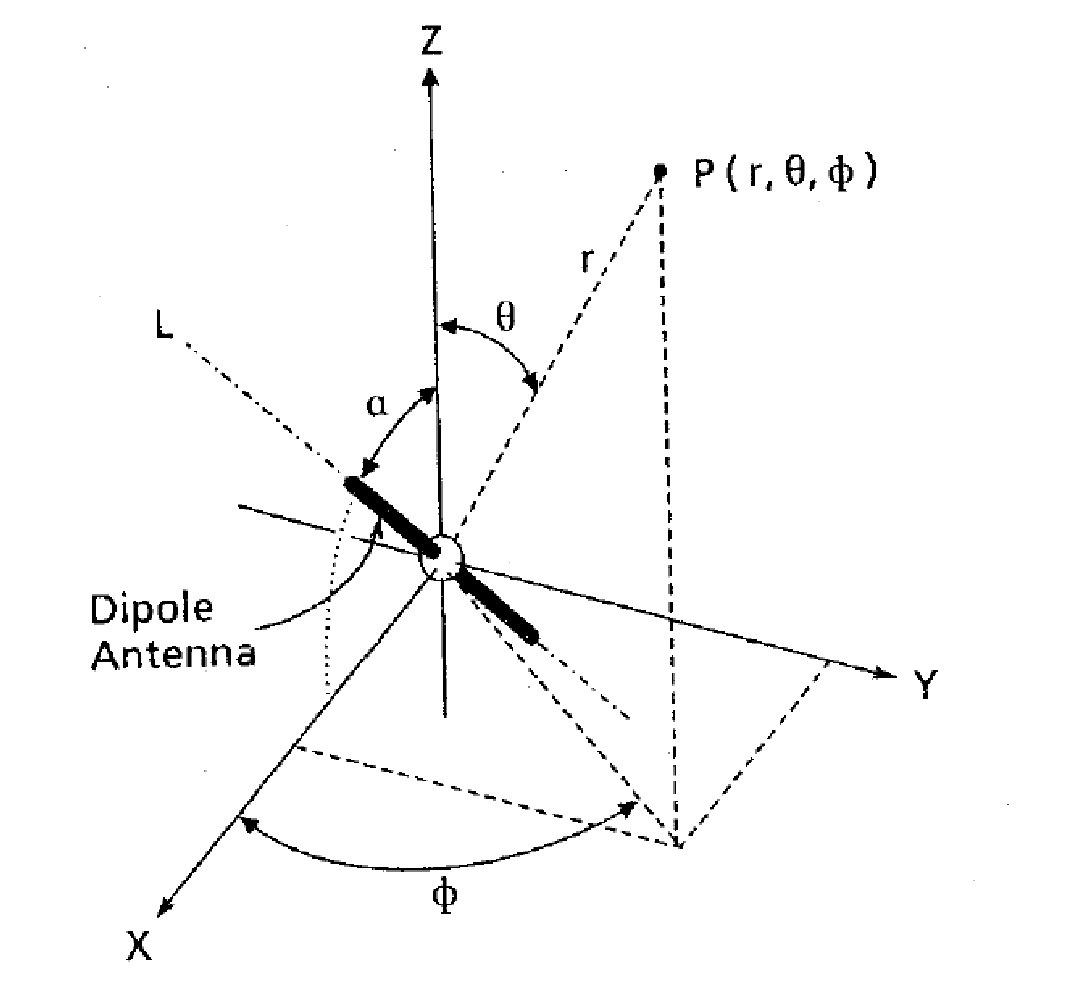
\includegraphics[width=10cm]{dipole_inclination.eps}
  \caption{Figure showing the angles involved in the dipole inclination and rotation (WRITE SOURCE)}
  \label{fig:dipole_inclination}
\end{figure}

The figures \ref{fig:street_nr}and \ref{fig:street_r} represent the situation in which the orientation of the antenna is rotated approximately 90 degrees. The important fact that relies on the different results of the MEG in both cases is the characteristic pattern of the power received in a street. The red ellipses in the figures represents the direction in which the power received is supposed to be higher, resulting in what can be called a 'cannon effect'. Given this, the orientation of the antenna is not negligible in the results and vary with the orientation.


\begin{figure}[!h]
  \centering
  \includegraphics[width=8cm]{street_nr.eps}
  \caption{Figure of the antenna with orientation to $\varphi=0$}
  \label{fig:street_nr}
\end{figure}

\begin{figure}[!h]
  \centering
  \includegraphics[width=8cm]{street_r.eps}
  \caption{Figure of the antenna with different orientation (approximately $\varphi=90$)}
  \label{fig:street_r}
\end{figure}



\chapter{MM6 - Dynamic Spectrum Access and Cognitive Radio}
This mini module is an introduction to the principal of \textit{Cognitive Radio}. The idea behind the concept is to distribute  the access to the medium/spectrum in a dynamic way. \\

\textit{From Wikipedia, the free encyclopedia}\\
A cognitive radio is an intelligent radio that can be programmed and configured dynamically. Its transceiver is designed to use the best wireless channels in its vicinity. Such a radio automatically detects available channels in wireless spectrum, then accordingly changes its transmission or reception parameters to allow more concurrent wireless communications in a given spectrum band at one location. This process is a form of dynamic spectrum management.

\section{Choice of Sharing Strategy}
In order to be able to access the spectrum in a dynamic way different strategies can be used one of them is simply to divide the spectrum in a way according to the changing need from the different users. This could either be in time or frequency. The problem in doing this is that you do not utilize the complete spectrum for the different users giving that efficiency is lost.\\

As an example can be used \figref{fig:TimeSlots} where there is unused time in between bursts of transmission, these could be used by a secondary system.  
\begin{figure}[!h]
  \centering
  \includegraphics[width=8cm]{TimeSlots.eps}
  \caption{Spectrum use over time}
  \label{fig:TimeSlots}
\end{figure}

However this is as mentioned not the best way of managing the spectrum as the burst of transmission from the primary transmitter could not be periodic or in varying length. If this is the case and the secondary transmitter transmit while the primary transmitter is also transmitting then interference will occur. Due to this a balance of what interference can be allowed have to be made. This can be illustrated by the following:
\begin{figure}[!h]
  \centering
  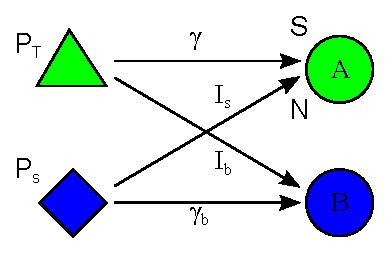
\includegraphics[width=8cm]{InterferenceFun.eps}
  \caption{Illustration of interference}
  \label{fig:InterferenceFun}
\end{figure}

In \figref{fig:InterferenceFun} $A$ and $B$ is the receiving nodes. $P_T$ is the primary transmitter and $P_S$ is the secondary transmitter. $\gamma$ and $\gamma_b$ is the attenuation (path-loss) from the transmitters to the receiving nodes. $I_S$ and $I_b$ is respectively the interference from the two transmitters. \\

The signal to noise ratio (SNR) is as know the ration between the intended signal and the interference, also marked at \figref{fig:InterferenceFun} with $S$ and $N$, note that $N$ is the noise inherent in the system. Without interference then $P_T$ can be related to a signal intended at $A$ which can be described as:
\begin{flalign}
 && \frac{S}{N} =& \gamma & \label{eq:SNRsimple}
\end{flalign} 

Knowing the path-loss ($\gamma$) also enables us to find the maximum (full) capacity of the channel using Shannon as follows:
\begin{flalign}
 && C_{full} =& \log_2(1+\gamma) & \label{eq:ShannonLimit}
\end{flalign} 

When we introduce the interference as shown in \figref{fig:InterferenceFun} instead of the SNR we will have to use the signal to interference ration (SINR). Which can be described as:
\begin{flalign}
 && SINR =& \frac{S}{I_S+N} & \label{eq:SINRsimple}
\end{flalign} 

If we then where to omit the noise ($N$) as this is something we cant do anything about in contrary to the interference ($I_S$) we could scale the expression \ref{eq:SINRsimple} with the noise as follows: 
\begin{flalign}
 && SINR =& \frac{S}{\frac{I_S}{N}+N} & 
\end{flalign}

Then remembering \equref{eq:SNRsimple} and introducing that $\beta = \frac{I_S}{N}$ we can write:
\begin{flalign}
 && SINR =& \frac{\gamma}{\beta+1} & \label{eq:SINRwithBeta}
\end{flalign}

With this we could again use Shannon to write up the capacity of the channel as follows:
\begin{flalign}
 && C_{interfered} =& \log_2\left(1+\frac{\gamma}{\beta+1}\right) & \label{eq:ShannonLimitSINR}
\end{flalign} 

The rate the system can operate at is determined by the capacity giving...

\chapter{MM7 - CDMA systems}
\section{Exercise 1} \label{sec:mm8_Ex1}
\textit{A list of parameters of a Wireless LAN air-interface (IEEE 802.11a) using OFDM is given below:
\begin{itemize}
 \item 64 subcarriers, 48 for data, 4 for pilots and 12 null subcarriers.
 \item Symbol duration 4 $\mu$s.
 \item Cyclic prefix 0.8 $\mu$s.
 \item Modulation: BPSK, QPSK, 16-QAM, 64-QAM
 \item Convolutional coding with rate 1/2 ; 2/3 ; 3/4
 \item System bandwidth 20MHz
 \item Bit rates of 6, 12, 18, 24, 36, 48 and 54Mbps
\end{itemize}
Calculate the following parameters:}


\subsection{1)}
\textit{FFT time-period}
\begin{flalign} 
 && T_{symbol} =& T_{G} + T_{FFT} & \\
 && T_{FFT} =& T_{symbol} - T_{G} & \\
\end{flalign}
With $T_{symbol}$ = 4 $\mu$s and $T_{G}$ = 0.8 $\mu$s
\begin{flalign}
 && T_{FFT} =& 4 - 0.8 & \\ 
 &&  =& 3.2 & [\SI{}{\micro\second}] & \label{eq:mm8_ex1_q1}
\end{flalign}

\subsection{2)}
\textit{Sampling frequency}
For the sampling frequency in baseband, each subcarrier needs to be extracted. 
\begin{flalign}
&& F_{S} =& \frac{N_{sub}}{T_{FFT}} &
\end{flalign}
$N_{sub}$ = 64 and $T_{FFT}$ from \equref{eq:mm8_ex1_q1}
\begin{flalign}
&& F_{S}=& 20 & [\SIf{}{\mega\hertz}]
\end{flalign}

\subsection{3)}
\textit{Sampling duration}
The sampling duration is equal to the time-period $T_{FFT}$ because the CP should be avoided from the synchronization.
\begin{flalign}
&& T_{S} =& T_{FFT} &
\end{flalign}

\subsection{4)}
\textit{Number of samples in the guard interval}
With a sampling frequency of 20MHz and a duration of the guard interval of 0.8$\mu$s
\begin{flalign}
&& NS_{GI} =& F_{S} \cdot T_{GI} &\\
&& =& 16 & 
\end{flalign}

\subsection{5)}
\textit{Subcarrier frequency spacing}
The spacing between the subcarriers should correspond to:
\begin{flalign}
 && F_{spacing} =& \frac{1}{T_{FFT}} &
 && =& 16 &
\end{flalign}


\subsection{6)}
\textit{For different data rates, different coding scheme and different combination of modulation scheme, calculate}

\subsubsection*{a)} 
\textit{Coded bits per subcarriers}
The coded bits,$C_{b}$, can be calculated by 
\begin{flalign}
&& C_{bsc} =& log_{2}(M)&
\end{flalign}
Where M is the order 
\\
For BPSK the coded bits per subcarrier is: 
\begin{flalign}
&& C_{bsc(BPSK)} =& 1&
\end{flalign}
For QPSK the coded bits per subcarrier is: 
\begin{flalign}
&& C_{bsc(QPSK)} =& 2&
\end{flalign}
For 16QAM the coded bits per subcarrier is: 
\begin{flalign}
&& C_{bsc(16QAM)} =& 4&
\end{flalign}
For 64QAM the coded bits per subcarrier is: 
\begin{flalign}
&& C_{bsc(64QAM)} =& 6&
\end{flalign}

\subsubsection*{b)} 
\textit{Coded bits per OFDM symbol}
\begin{flalign}
&& C_{bsy} =& N_{data carriers} \cdot log_{2}(M)&
\end{flalign}
For BPSK the coded bits per subcarrier is: 
\begin{flalign}
&& C_{bsy(BPSK)} =& 1 \cdot 48& \\
&& =& 48 &
\end{flalign}
For QPSK the coded bits per subcarrier is: 
\begin{flalign}
&& C_{bsy(QPSK)} =& 2 \cdot 48& \\
&& =& 96 &
\end{flalign}
For 16QAM the coded bits per subcarrier is: 
\begin{flalign}
&& C_{bsy(16QAM)} =& 4 \cdot 48& \\
&& =&  192& 
\end{flalign}
For 64QAM the coded bits per subcarrier is: 
\begin{flalign}
&& C_{bsy(64QAM)} =& 6 \cdot 48& \\
&& =& 288 &
\end{flalign}

\subsubsection*{c)} 
\textit{Data bits per OFDM symbol}

\section{Exercise 2} \label{sec:mm8_Ex1}
\textit{Show that the last $N$ samples of the circular convolution with the cyclic prefix are equal to the $N$ samples of the linear convolution when an empty cyclic prefix is used.}\\

For this we used \cite[p.~384]{lit:goldsmith} as reference. We want at the receiver to have something that looks like the circular convolution of the channel with the signal we want to obtain because if the channel is known, then, the wanted signal can be easily found. However we have the problem that the channel has the effect over any sent signal of producing a linear convolution. Mathematically we have 2 options, in theory we can modify $h[n]$ or the sent signal. However, practically, we do not have any control over the channel so we can only change the signal $x[n]$ to a certain $\tilde{x}[n]$, but what this $\tilde{x}[n]$ should be?.

If we add a cyclic prefix as long as the memory of the channel, length $\mu$ to the signal $x[n]$, this is $\tilde{x}[n]=x[n]_{N}$, for $-\mu \leq n \leq N-1$ then, after sending that new signal through the channel, we get in the receiver something that looks like the circular convolution that we want as it is shown in the followings equations.

\begin{flalign} 
 && y[n] =& \tilde{x}[n] \ast h[n] & \\
 &&      =& \sum_{k=0}^\mu h[n]\,\tilde{x}[n-k]& \\
 &&      =& \sum_{k=0}^\mu h[n]\,x[n-k]_{N} \\
 &&      =& \,x[n]\circledast h[n]&
\end{flalign}

This is true because the third equality follows from the fact that, for $0 \leq k \leq \mu$, $\tilde{x}[n-k]=x[n-k]_{N}$ for $0 \leq n \leq N-1$.

\chapter{MM8 - OFDM}
\section{Exercise 1} \label{sec:mm8_Ex1}
\textit{A list of parameters of a Wireless LAN air-interface (IEEE 802.11a) using OFDM is given below:
\begin{itemize}
 \item 64 subcarriers, 48 for data, 4 for pilots and 12 null subcarriers.
 \item Symbol duration 4 $\mu$s.
 \item Cyclic prefix 0.8 $\mu$s.
 \item Modulation: BPSK, QPSK, 16-QAM, 64-QAM
 \item Convolutional coding with rate 1/2 ; 2/3 ; 3/4
 \item System bandwidth 20MHz
 \item Bit rates of 6, 12, 18, 24, 36, 48 and 54Mbps
\end{itemize}
Calculate the following parameters:}


\subsection{1)}
\textit{FFT time-period}
\begin{flalign} 
 && T_{symbol} =& T_{G} + T_{FFT} & \\
 && T_{FFT} =& T_{symbol} - T_{G} & \\
\end{flalign}
With $T_{symbol}$ = 4 $\mu$s and $T_{G}$ = 0.8 $\mu$s
\begin{flalign}
 && T_{FFT} =& 4 - 0.8 & \\ 
 &&  =& 3.2 & [\SI{}{\micro\second}] & \label{eq:mm8_ex1_q1}
\end{flalign}

\subsection{2)}
\textit{Sampling frequency}
For the sampling frequency in baseband, each subcarrier needs to be extracted. 
\begin{flalign}
&& F_{S} =& \frac{N_{sub}}{T_{FFT}} &
\end{flalign}
$N_{sub}$ = 64 and $T_{FFT}$ from \equref{eq:mm8_ex1_q1}
\begin{flalign}
&& F_{S}=& 20 & [\SIf{}{\mega\hertz}]
\end{flalign}

\subsection{3)}
\textit{Sampling duration}
The sampling duration is equal to the time-period $T_{FFT}$ because the CP should be avoided from the synchronization.
\begin{flalign}
&& T_{S} =& T_{FFT} &
\end{flalign}

\subsection{4)}
\textit{Number of samples in the guard interval}
With a sampling frequency of 20MHz and a duration of the guard interval of 0.8$\mu$s
\begin{flalign}
&& NS_{GI} =& F_{S} \cdot T_{GI} &\\
&& =& 16 & 
\end{flalign}

\subsection{5)}
\textit{Subcarrier frequency spacing}
The spacing between the subcarriers should correspond to:
\begin{flalign}
 && F_{spacing} =& \frac{1}{T_{FFT}} &
 && =& 16 &
\end{flalign}


\subsection{6)}
\textit{For different data rates, different coding scheme and different combination of modulation scheme, calculate}

\subsubsection*{a)} 
\textit{Coded bits per subcarriers}
The coded bits,$C_{b}$, can be calculated by 
\begin{flalign}
&& C_{bsc} =& log_{2}(M)&
\end{flalign}
Where M is the order 
\\
For BPSK the coded bits per subcarrier is: 
\begin{flalign}
&& C_{bsc(BPSK)} =& 1&
\end{flalign}
For QPSK the coded bits per subcarrier is: 
\begin{flalign}
&& C_{bsc(QPSK)} =& 2&
\end{flalign}
For 16QAM the coded bits per subcarrier is: 
\begin{flalign}
&& C_{bsc(16QAM)} =& 4&
\end{flalign}
For 64QAM the coded bits per subcarrier is: 
\begin{flalign}
&& C_{bsc(64QAM)} =& 6&
\end{flalign}

\subsubsection*{b)} 
\textit{Coded bits per OFDM symbol}
\begin{flalign}
&& C_{bsy} =& N_{data carriers} \cdot log_{2}(M)&
\end{flalign}
For BPSK the coded bits per subcarrier is: 
\begin{flalign}
&& C_{bsy(BPSK)} =& 1 \cdot 48& \\
&& =& 48 &
\end{flalign}
For QPSK the coded bits per subcarrier is: 
\begin{flalign}
&& C_{bsy(QPSK)} =& 2 \cdot 48& \\
&& =& 96 &
\end{flalign}
For 16QAM the coded bits per subcarrier is: 
\begin{flalign}
&& C_{bsy(16QAM)} =& 4 \cdot 48& \\
&& =&  192& 
\end{flalign}
For 64QAM the coded bits per subcarrier is: 
\begin{flalign}
&& C_{bsy(64QAM)} =& 6 \cdot 48& \\
&& =& 288 &
\end{flalign}

\subsubsection*{c)} 
\textit{Data bits per OFDM symbol}

\section{Exercise 2} \label{sec:mm8_Ex1}
\textit{Show that the last $N$ samples of the circular convolution with the cyclic prefix are equal to the $N$ samples of the linear convolution when an empty cyclic prefix is used.}\\

For this we used \cite[p.~384]{lit:goldsmith} as reference. We want at the receiver to have something that looks like the circular convolution of the channel with the signal we want to obtain because if the channel is known, then, the wanted signal can be easily found. However we have the problem that the channel has the effect over any sent signal of producing a linear convolution. Mathematically we have 2 options, in theory we can modify $h[n]$ or the sent signal. However, practically, we do not have any control over the channel so we can only change the signal $x[n]$ to a certain $\tilde{x}[n]$, but what this $\tilde{x}[n]$ should be?.

If we add a cyclic prefix as long as the memory of the channel, length $\mu$ to the signal $x[n]$, this is $\tilde{x}[n]=x[n]_{N}$, for $-\mu \leq n \leq N-1$ then, after sending that new signal through the channel, we get in the receiver something that looks like the circular convolution that we want as it is shown in the followings equations.

\begin{flalign} 
 && y[n] =& \tilde{x}[n] \ast h[n] & \\
 &&      =& \sum_{k=0}^\mu h[n]\,\tilde{x}[n-k]& \\
 &&      =& \sum_{k=0}^\mu h[n]\,x[n-k]_{N} \\
 &&      =& \,x[n]\circledast h[n]&
\end{flalign}

This is true because the third equality follows from the fact that, for $0 \leq k \leq \mu$, $\tilde{x}[n-k]=x[n-k]_{N}$ for $0 \leq n \leq N-1$.

\part{Daniel - Cooperation in Wireless Networks}
\chapter{MM9 - Network Coding for Wireless Networks}
Advantages of using directive antennas -> space as 4th access/multiplex dimension\\

Beam space vs signal space methods (forward-reverse link sensitivity)\\

User tracking (link) vs traffic tracking (coverage)\\

Access vs interference suppression

\section{Symmetric Alice and Bob}
\textit{In this exercise, the flows between Alice and Bob are symmetric, similar to the discussions in class, meaning that each source provides a throughput of R to the system. This means that the system load at any point will be 2R. The task is to give derive the analytical expressions for the throughput for the case of not using network coding and the case of using network coding in the presence of a Medium Access Control (MAC) mechanism that provides fair access to the channel. Assume no losses occur in the different communication channels.}

\subsection{Exercise 1: Throughput Without Network Coding}
\textit{It is recommended to attack this problem in three stages. First, identify the three key regions of operation when not using network coding justifying your answer. Second, derive analytical expressions for the total system throughput, i.e., the addition of the end-to-end throughput of the connection from Alice to Bob and from Bob to Alice, versus the system load (2R). Finally, plot the total system throughput versus the system load.}\\

In the case without network coding the Relay sends the double amount of data compared to Alice and Bob until the maximum capacity is reached which is 0.5 R with a $50 \%$ of the load system, where A and B are sending $\dfrac{1}{4}R$. After this point the throughput will drop until $\dfrac{1}{3} R $ with a corresponding load of $66 \%$. After this point the throughput will stay stable at that value. To have a better understanding a plot (\figref{fig:throughput_WNC}) of the throughput vs the load of the system is made.
\begin{figure}[!h]
  \centering
  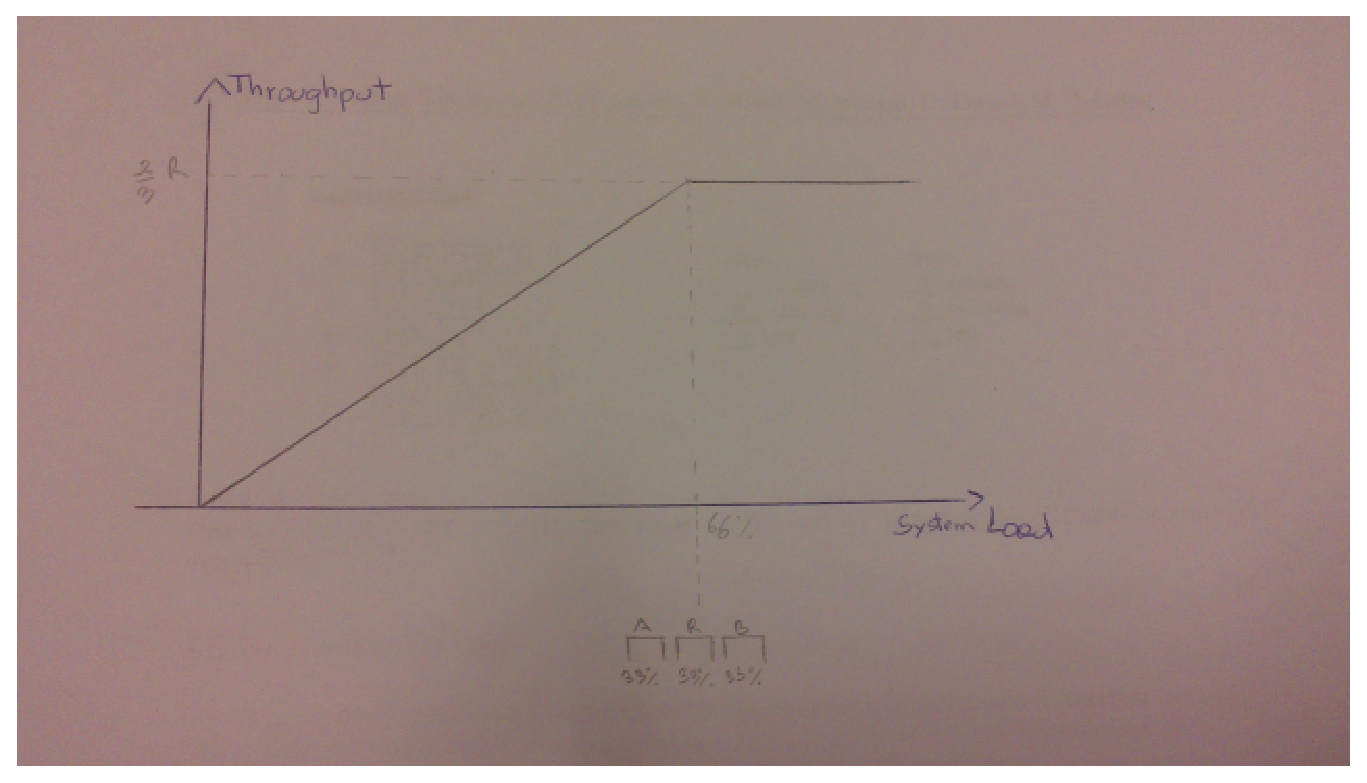
\includegraphics[width=15cm]{throughput_WNC.eps}
  \caption{throughput without NC}
  \label{fig:throughput_WNC}
\end{figure}

\subsection{Exercise 2: Throughput With Network Coding}
\textit{Repeat the steps of the previous question but using inter-session network coding at the relay. How many regions of operations are there and why?}\\

For the Network Coding the scenario is a bit different. The relays in this case sends the same amount of data as Alice and Bob. The throughput will grow until the maximum capacity is reached ($\dfrac{2}{3} R $), since each node is able to send $\dfrac{1}{3} R $ and it will stay stable with a $66 \%$ of the system load.  

\begin{figure}[!h]
  \centering
  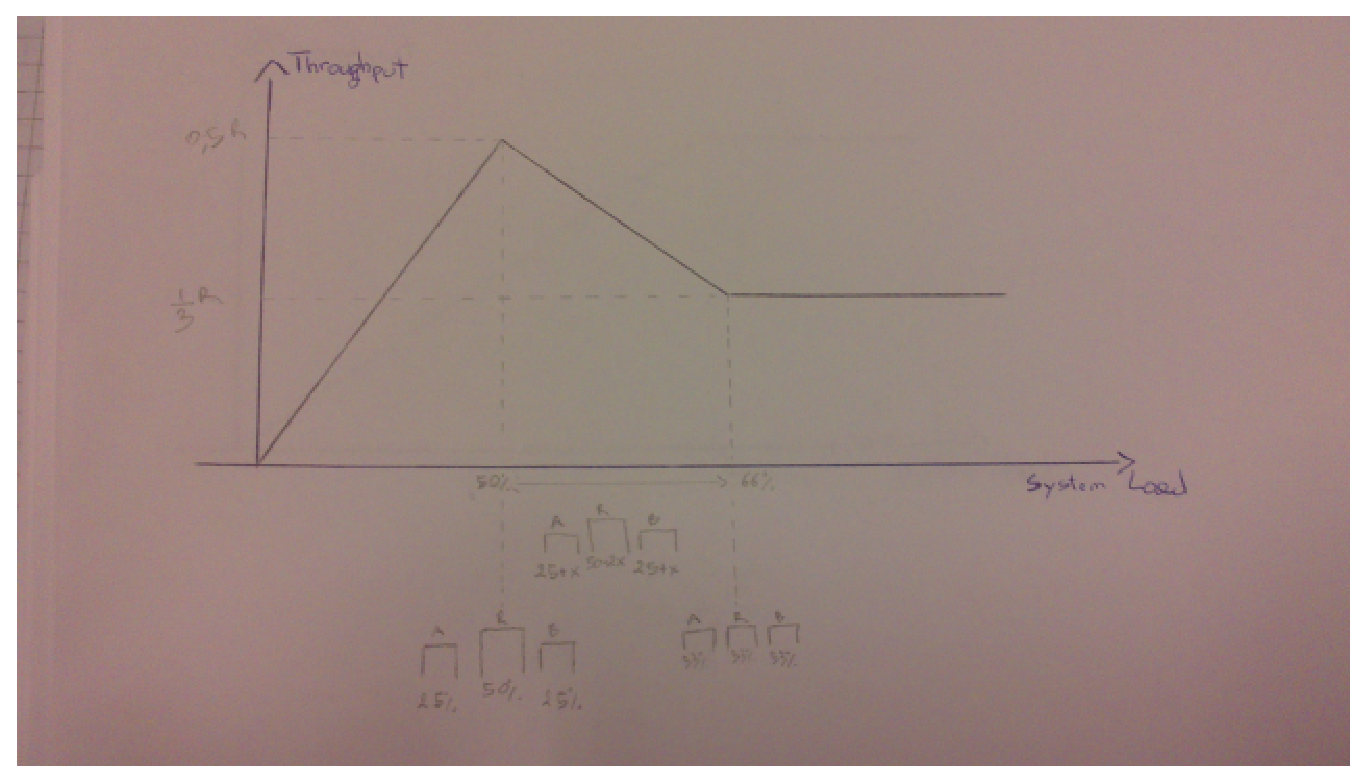
\includegraphics[width=15cm]{throughput_NC.eps}
  \caption{throughput with NC}
  \label{fig:throughput_NC}
\end{figure}

\section{Bidirectional Cross}
\textit{An elementary topology where network coding can provide interesting benefits is the bidirectional cross, where we distinguish between three cases:}\\

\begin{figure}[!h]
  \centering
  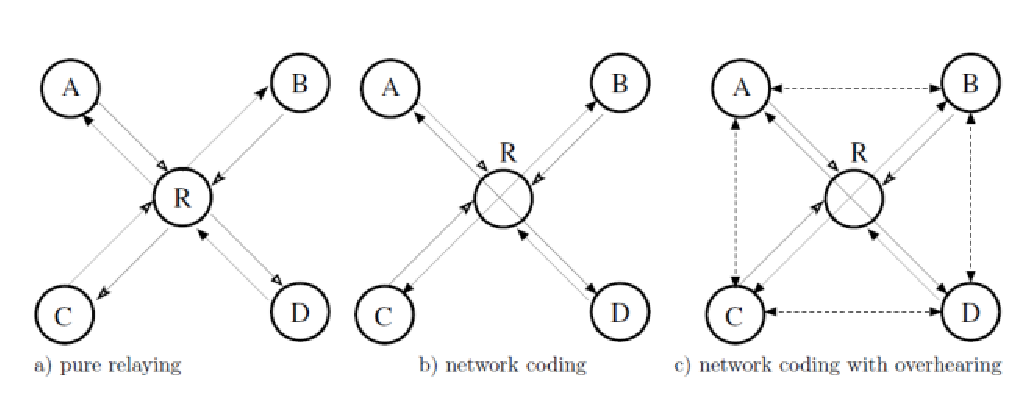
\includegraphics[width=15cm]{Bidirectional_Cross.eps}
  \caption{Bidirectional Cross}
  \label{fig:Bidirectional_Cross}
\end{figure}

\textit{Specifically, the cases are (a) pure relaying, where packets are not combined, (b) network coding, where two packets are combined, and (c) network coding with overhearing, where the relay combines four packets.}


\subsection{Exercise 3: Activities.}
\textit{Give the activities for each node in the topology for cases (a), (b), and (c). The possible activities for each node are idle, receive, and send. The following tables are intended as a help to construct the respective activity plots.}\\

Something...

\subsection{Exercise 2: Throughput With Network Coding}
\textit{Repeat the steps of the previous question but using inter-session network coding at the relay. How many regions of operations are there and why?}

\subsubsection{(a) Pure Relaying}
\begin{figure}[!h]
  \centering
  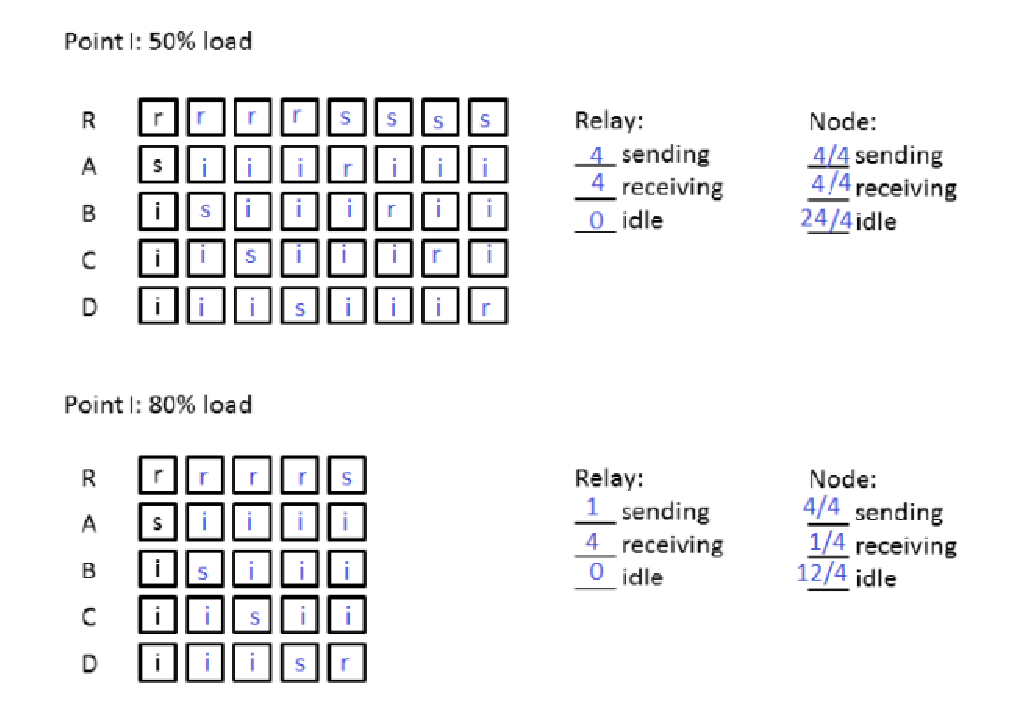
\includegraphics[width=15cm]{Pure_relaying.eps}
  \caption{Pure Relaying}
  \label{fig:Pure_relaying}
\end{figure}
\newpage
\subsubsection{(b) Network Coding}
\begin{figure}[!h]
  \centering
  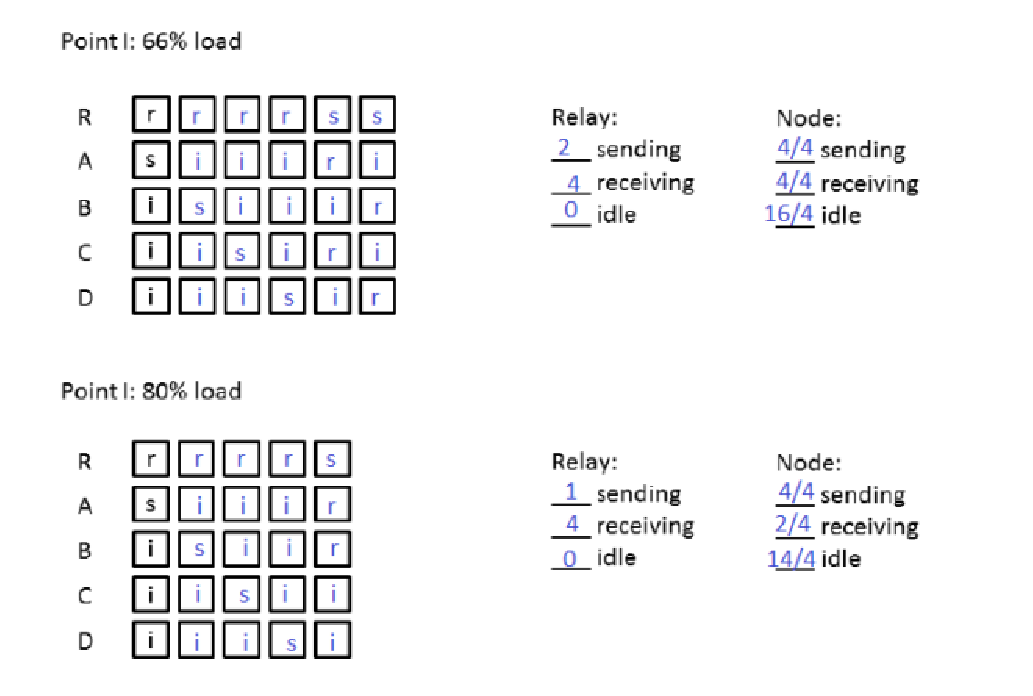
\includegraphics[width=15cm]{network_coding.eps}
  \caption{Network Coding}
  \label{fig:network_coding}
\end{figure}
\newpage
\subsubsection{(c) Network Coding with Overhearing}
\begin{figure}[!h]
  \centering
  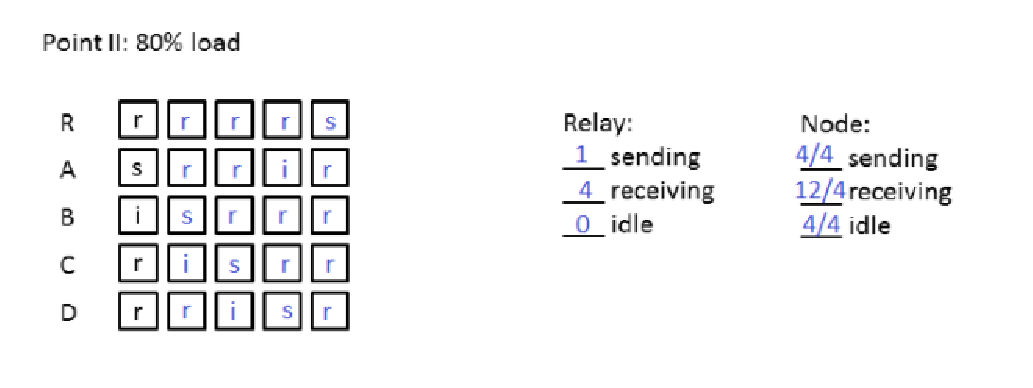
\includegraphics[width=15cm]{network_coding_overhearing.eps}
  \caption{Network Coding Overhearing}
  \label{fig:network_coding_overhearing}
\end{figure}

\subsection{Exercise 4: Throughput}
\textit{Give the total throughput for the three cases (a), (b), and (c), including the plot and the analytical expressions}\\
\begin{pitemize}
\item For the case (a) the throughput is the $100 \%$ of the load ($50 \%$) because all the node receiving the packets from the relay R. \\In the case where the load is $80 \%$ the throughput is $25 \%$ of the $80 \%$ because only one note receive the packet.
\item For the case (b) with a load of $66\%$ the throughput is $100 \%$ of the $66\%$ because the relay in two operations forward the packet to the all nodes. \\ In the case where the load is $80 \%$ the throughput of the this specific load is $50 \%$ because only two receiving the packet.
\item For the case (c) the throughput is the $100 \%$ of the load because all nodes receiving the package. 
\end{pitemize}

\section{Intra session Coding}
\textit{Consider a source that will send 3 data packets (P1, P2, P3) with n bits each to a destination using RLNC with GF(2). A coded packet CP is generated by a linear combination of the original data packets, i.e.,}

\subsection{Exercise 5: Parameters }
\textit{What is the field size and the generation size in this problem?}\\

Something...

\subsection{Exercise 2: Throughput With Network Coding}
\textit{Assuming that the destination has no coded packets at the beginning, what is the probability of a linear combination not being useful? Use the following table that represents the coding coefficients ci of each original packet Pi to identify which case(s) are useful or not. Calculate the probability knowing that each case is equally likely.}\\

\begin{figure}[!h]
  \centering
  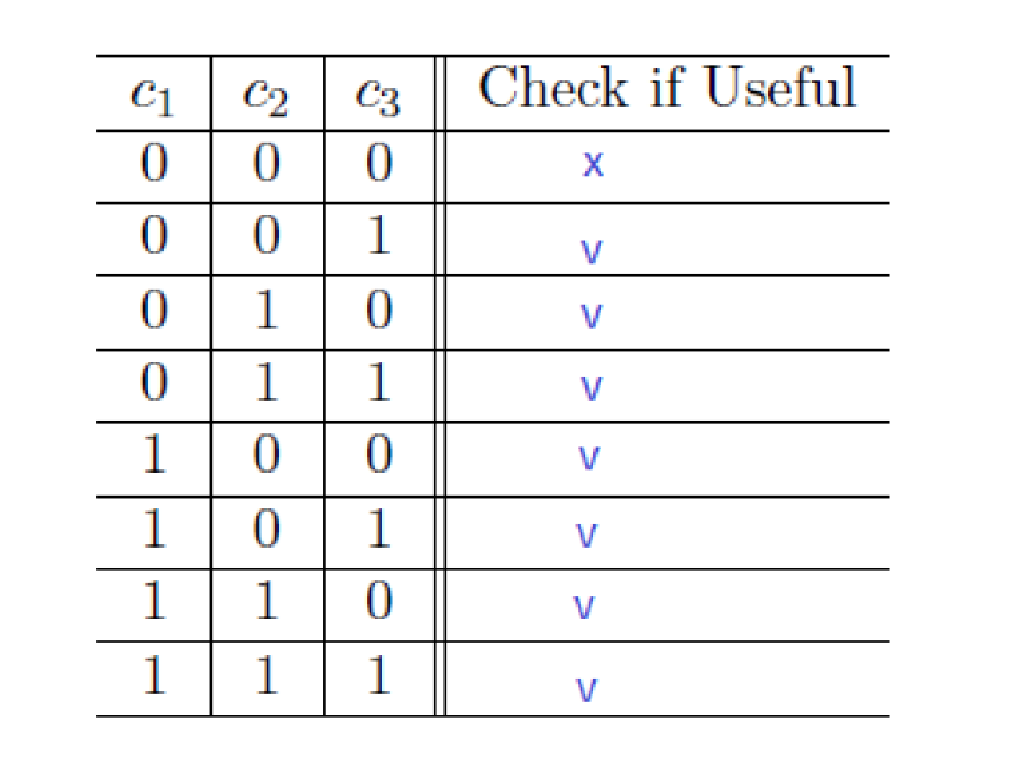
\includegraphics[width=8cm]{Intra_session_1.eps}
  \caption{}
  \label{fig:Intra_session_1}
\end{figure}
The probability knowing that each case is equally likely is $P=\frac{7}{8}$.\\

\textit{Assuming that one coded packet has arrived to the destination with coding coefficients (0, 1, 1), calculate again the probability of a new incoming coded packet being useful to the receiver. Use the following table for help.}\\

\begin{figure}[!h]
  \centering
  \includegraphics[width=8cm]{Intra_session_2.eps}
  \caption{}
  \label{fig:Intra_session_2}
\end{figure}
The probability knowing that each case is equally likely is $P=\frac{6}{8}=\frac{3}{4}$.\\
\textit{Assuming that two coded packets have arrived to the destination with coding coefficients (0, 1, 1) and (1, 1, 0), calculate again the probability of a new incoming coded packet being useful to the receiver. Note that this corresponds to the probability of receiving the last useful coded packet before being able to decode. Use the following table for help.}\\

\begin{figure}[!h]
  \centering
  \includegraphics[width=8cm]{Intra_session_3.eps}
  \caption{}
  \label{fig:Intra_session_3}
\end{figure}
The probability knowing that each case is equally likely is $P=\frac{4}{8}=\frac{1}{2}$.\\
\subsubsection{What conclusions can you derive from these results?}

\subsubsection{When the generation size is larger, will the probability of receiving the last coded packet before decoding change?}



\chapter{MM10 - Basics of Cooperation, Application, and Device Requirements}
Advantages of using directive antennas -> space as 4th access/multiplex dimension\\

Beam space vs signal space methods (forward-reverse link sensitivity)\\

User tracking (link) vs traffic tracking (coverage)\\

Access vs interference suppression

\section{Problem 1 - Simulations with NETLOGO}
Install the program and do the following. (http://ccl.northwestern.edu/netlogo/)
\subsection{Compare the revenue for 10 TIT-FOR-TAT and 10 DEFECT turtles}

The simulation is setup in the software and the resulting plot is shown in \figref{fig:10tft_10def-jpg}.
\begin{figure}[!h]
  \centering
  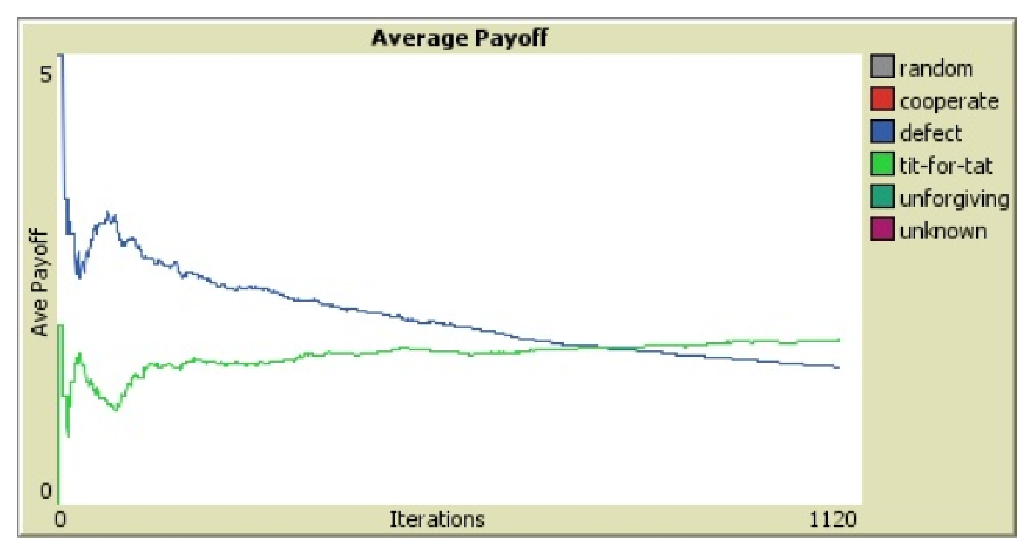
\includegraphics[width=10cm]{10tft_10def-jpg.eps}
  \caption{Simulation for 10 TIT-FOR-TAT and 10 DEFECT turtles running 1120 iterations}
  \label{fig:10tft_10def-jpg}
\end{figure}

From \figref{fig:10tft_10def-jpg} it can be seen that the intersect point between the two strategies is after 760 moves in payoff point 1.74 and the payoff is settling for TIT-FOR-TAT at 1.94 and for DEFECT at 1.\\

From the plot it can be seen that using the defect strategic gives the biggest pay-off in the beginning but after 760 iterations the tit for tat strategy is giving best pay-off. This is telling us that for a short interaction with other nodes the largest gain can come from the defect strategy but in the long term tit for tat is better.   

\subsection{Use all six strategies in NetLogo for 10 turtles and comment on the results}

Again the simulation is setup in the software and the results is plotted in \figref{fig:all10turtles-jpg}. This plot can be difficult to read therefore a plot of the first 715 iterations is shown in \figref{fig:all10turtles_start-jpg} and for showing the settling \figref{fig:all10turtles_end-jpg}. 

\begin{figure}[!h]
  \centering
  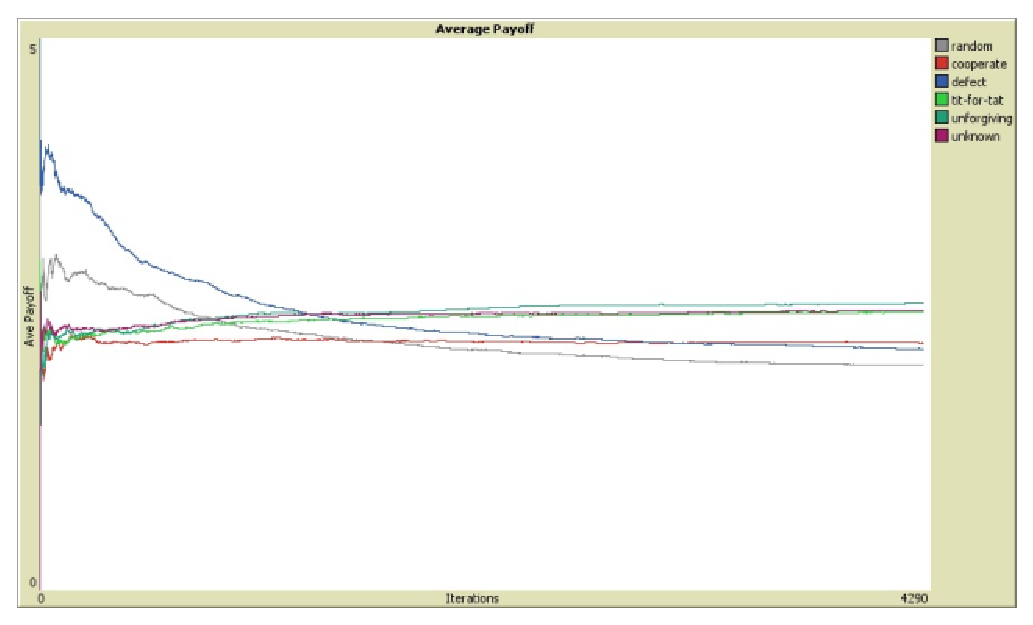
\includegraphics[width=12cm]{all10turtles-jpg.eps}
  \caption{All 10 strategies simulated with 10 turtles}
  \label{fig:all10turtles-jpg}
\end{figure}


\begin{figure}[!h]
  \centering
  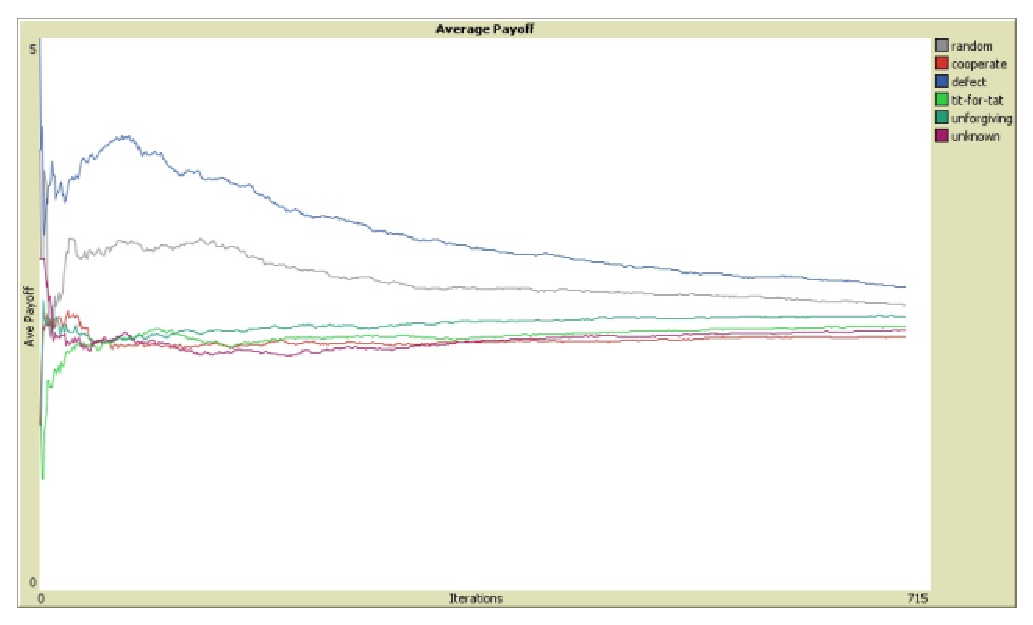
\includegraphics[width=12cm]{all10turtles_start-jpg.eps}
  \caption{First iterations of the simulations}
  \label{fig:all10turtles_start-jpg}
\end{figure}
This shows which strategy is the best for a short interaction with other nodes. Giving the largest pay-off in the beginning of the iterations. 

\begin{figure}[!h]
  \centering
  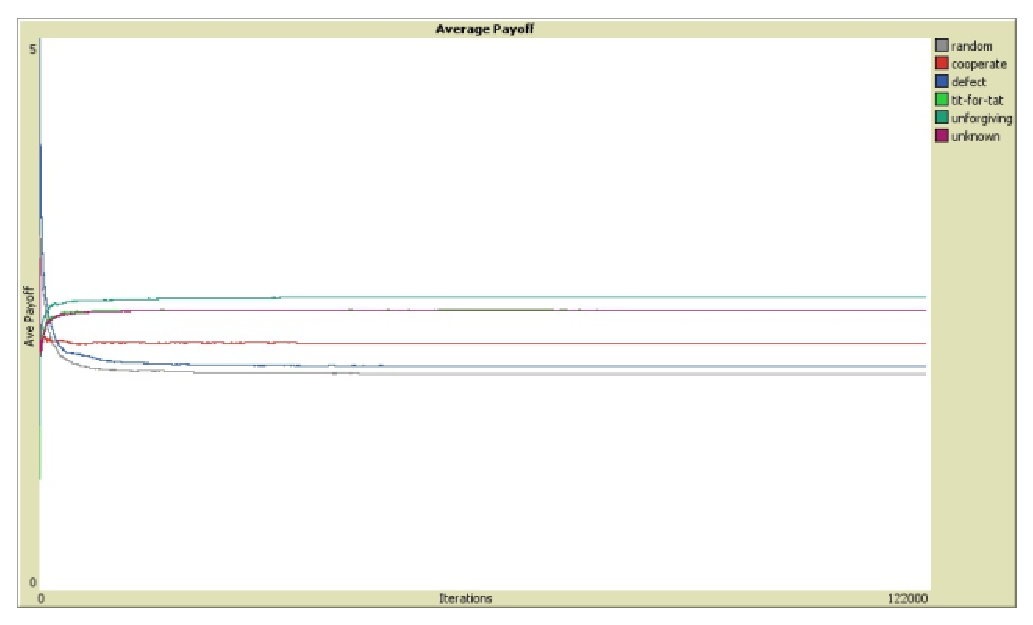
\includegraphics[width=12cm]{all10turtles_end-jpg.eps}
  \caption{Settling effect of the simulation}
  \label{fig:all10turtles_end-jpg}
\end{figure}
\FloatBarrier

The different strategies settles at the following pay-off rate:
\begin{pitemize}
	\item Random = 1.957
	\item Unforgiving = 2.657
	\item Unknown = 2.532
	\item Defect = 2.026
	\item Cooperate = 2.234
	\item Tit for Tat = 2.534
\end{pitemize}


\section{Problem 1 - Analytical expressions}
\textit{Derive analytical expressions for different tactics. }\\

The pay off from the different tactics is given by the following:
\begin{center}
  \begin{tabular}{ c | c | c }
      			& Cooperate & Defect 	\\ \hline
    Cooperate 	& 3/3	 	& 0/5 		\\ \hline
    Defect		& 5/0 		& 1/1 		\\
    \hline
  \end{tabular}
\end{center}
The expression to use here is given by:
\begin{flalign}
 && \texttt{PayOff}=& \frac{\texttt{[Total \# of same tactic]}\cdot \texttt{[Point]} + \texttt{[Total \# of different tactic]}\cdot \texttt{Point}}{\texttt{Total \# of nodes}} &
\end{flalign}
\subsection{10 TIT for TAT and 10 DEFECT}
For this the expression can be written like:
\begin{flalign}
 && TfT=& \frac{9\cdot 3 + 10\cdot 1}{19} =1.95 &
\end{flalign}

\begin{flalign}
 && Defect=& \frac{9\cdot 1 + 10\cdot 1}{19} =1 &
\end{flalign}

I can be noted that this is the same (almost) as the values found in the simulations shown in \figref{fig:10tft_10def-jpg}.

\subsection{10 COOPERATE and 10 DEFECT}
\begin{flalign}
 && Coop=& \frac{9\cdot 3 + 10\cdot 0}{19} =1.42 &
\end{flalign}

\begin{flalign}
 && Defect=& \frac{9\cdot 1 + 10\cdot 5}{19} =3.1 &
\end{flalign}

\subsection{T TIT for TAT, D DEFECT and C COOPERATE}
Tit for tat:
\begin{flalign}
 && TfT=& \frac{(T-1)\cdot 3 + C\cdot 3 + D\cdot 1}{T+D+C-1} =\frac{3\left(T+C-1\right)+D}{T+D+C-1} &
\end{flalign}

Cooperate:
\begin{flalign}
 && Coop=& \frac{T\cdot 3 + (C-1)\cdot 3 }{T+D+C-1} =\frac{3\left(T+C-1\right)}{T+D+C-1} &
\end{flalign}

Defect:
\begin{flalign}
 && Defect=& \frac{T\cdot 1 + C\cdot 5 + (D-1)\cdot 1}{T+D+C-1} =\frac{5\cdot C+T+D}{T+D+C-1} &
\end{flalign}

\section{Problem 2 - Topology}

\chapter{MM11 - Energy and Data Rates}
Advantages of using directive antennas -> space as 4th access/multiplex dimension\\

Beam space vs signal space methods (forward-reverse link sensitivity)\\

User tracking (link) vs traffic tracking (coverage)\\

Access vs interference suppression

\section{Problem 1}
\textit{Using the overhearing cross topology for NC, consider that transmission of a packet has a cost of $E_t$ and reception of a packet a cost of $E_r$. Assume initially no losses in the links.}

\subsection{a) - Calculate the total energy used to deliver one packet from each }





\subsection{b) - x }





\subsection{c) - x }






\subsection{d) - x }






\subsection{e) - x }




\section{Problem 2}
\textit{Repeat problem 1 parts a)-d) considering the same topology, consider now that there is a cost for being idel, $E_{idel}$, and a cost for XOR'ing the data packets, $E_{XOR}$. How large would $E_{XOR}$ (as a function of the other energy terms) have to be for the network coding to be impractical in this setting.}\\

SOMETHING
\section{Problem 3}
\textit{Assuming a DVB-H system enhanced with short range communication technologies similar to the one studied in class but nodes attempting to watch one channel. Assume the transmit and receive power for short range communication is Ptsr and Prsr, respectively, and that the receive power from the cellular base station is Prc. Assume that n receivers are part of a cooperative cluster and that the loss probability of packets coming from the cellular base station and from other nodes in the cluster is ec and ed, respectively. Calculate the mean energy consumption for the following scenarios.}

\subsection{a)}
\textit{Nodes in the cooperative cluster nominate a cluster head that overhears transmissions from the base station and exchange packets to the others using unicast transmissions that rely on an ARQ mechanism.}\\
To calculate the energy the power needs to be related to time. So for transmission from base station to nodes the energy used is $E_{rc} = P_{rc} \cdot t_{1}$ and between the nodes $E_{rsr} = P_{rsr} \cdot t_{2}$ given the time for transmitting the data and receiving it is the same the energy for transmission is $E_{tsr} = P_{tsr} \cdot t_{2}$. The energy used for the cluster head to receive the packet is $E_{rch} = \frac{E_{rc}}{ec}$. The energy used for the cluster head to transmit to the rest of the clusters and for those to receive it using unicast is $E_{chc} = (n-1) \cdot \frac{(E_{tsr} + E_{rsr})}{ed}$. The total energy used to transmit the data from the base station to the cluster is 
\begin{flalign}
 && E_{total}=& E_{rch} + E_{chc}& \\
 && =& \frac{E_{rc}}{ec} +  (n-1) \cdot \frac{(E_{tsr} + E_{rsr})}{ed}&
\end{flalign}



\subsection{b)}
\textit{Nodes in the cooperative cluster receive directly from the base station.}\\
Same assumptions applies as in \textbf{a)} but here all nodes receives from the base station. So the energy used to transmit to all is 
\begin{flalign}
 && E_{total}=&n \cdot \frac{P_{rc} \cdot t}{ec} &
\end{flalign}


\part{Troels Part 2}
\chapter{MM12 - Network Performance-Cost-Energy}
Advantages of using directive antennas -> space as 4th access/multiplex dimension\\

Beam space vs signal space methods (forward-reverse link sensitivity)\\

User tracking (link) vs traffic tracking (coverage)\\

Access vs interference suppression

\section{Problem A}
\textit{You are to make a total cost of ownership (TCO) financial estimate to determine the direct and indirect costs of an indoor wireless system over an analysis period of 5 years.}\\

\textit{The system consists initially of 5 enterprise Femto base stations at a price tag of 500 Euros each and depreciation period of 7 years; the price erosion of the base station equipment is 6\% per year. In addition to the Femto base stations the system comprises a Femto gateway controller capable of handling up to 10 base stations; the gateway has a price tag of 50 Euros per connected base station and a depreciation period of 10 years. The base stations are connected to the gateway over an already existing Gigabit Ethernet network. The traffic from the gateway to the external network (backhaul) is carried over a leased fibre-optic connection, at a cost of 400 Euros per month. The installation cost per new Femto is 300 Euros and the annual service cost amounts to 20\% of the equipment cost; installation, service and leasing costs increase by 2\% annually.}\\

SOMETHING...\\

\textit{After 3 years, an additional 3 Femto base stations, with the same depreciation period of 7 years, are installed in the system.}\\

SOMETHING...\\

\textit{Detail the contributions to CAPEX, IMPEX and OPEX and calculate the TCO of this indoor wireless solution assuming a (risk and inflation compensated) interest rate of 5\%.}\\

SOMETHING...
\section{Problem B}
\textit{Anti collision - Aloha type exercise, As in A: but now try w one or more Aloha type protocols}\\

For this example we've considered the Slotted Aloha Protocol. We've done 2 different simulations, one with 3 time slots and another one with 4 slots.
\\
\\

\textbf{3 Slots}

\ptable{| c | c | c | c | c | c | c |}{ %
Person & Maria & Djam & Jesper & Pablo & Anders & Marika \\\hline
1st Iteration & Slot 3 & Slot 3 & \underline{\textbf{Slot 1}} & Slot 2 & Slot 3 & Slot 2 \\\hline
2nd Iteration & Slot 2 & \underline{\textbf{Slot 1}} & -- & Slot 2 & Slot 2 & Slot 2 \\\hline
3rd Iteration & Slot 1 & -- & -- & Slot 1 & Slot 3 & Slot 3 \\\hline
4th Iteration & \underline{\textbf{Slot 1}} & -- & -- & Slot 2 & Slot 2 & Slot 2 \\\hline
5th Iteration & -- & -- & -- & Slot 2 & Slot 2 & \underline{\textbf{Slot 1}} \\\hline
6th Iteration & -- & -- & -- & \underline{\textbf{Slot 3}} & \underline{\textbf{Slot 1}} & -- \\\hline
}{ID table for all persons}{tab1:mm13_prob_b}

\textbf{4 Slots}
\ptable{| c | c | c | c | c | c | c |}{ %
Person & Maria & Djam & Jesper & Pablo & Anders & Marika \\\hline
1st Iteration & Slot 2 & Slot 1 & Slot 1 & Slot 2 & \underline{\textbf{Slot 3}} & \underline{\textbf{Slot 4}} \\\hline
2nd Iteration & \underline{\textbf{Slot 2}} & Slot 4 & Slot 4 & Slot 4 & -- & -- \\\hline
3rd Iteration & -- & Slot 2 & Slot 2 & \underline{\textbf{Slot 1}} & -- & -- \\\hline
4th Iteration & -- & \underline{\textbf{Slot 3}} & \underline{\textbf{Slot 2}} & -- & -- & -- \\\hline
}{ID table for all persons}{tab1:mm13_prob_b2}

To complete statistically this part, we ran multiples simulations with the same parameters to obtain a more reliable results:

\ptable{| c | c | c | c |}{ %
Nº Slots Considered & 3 Slots & 4 Slots & 5 Slots \\\hline
Average Iterations Needed & 5.5 & 3.86 & 3.17 \\\hline
Average total slots & 16.5 & 15.44 & 15.85 \\\hline
}{ID table for all persons}{tab1:mm13_prob_b2}


\part{Patrick Part 3}
\chapter{MM13 - Passive radio communication (UHF RFID)}
Advantages of using directive antennas -> space as 4th access/multiplex dimension\\

Beam space vs signal space methods (forward-reverse link sensitivity)\\

User tracking (link) vs traffic tracking (coverage)\\

Access vs interference suppression

\section{Problem 1}
\textit{Using the overhearing cross topology for NC, consider that transmission of a packet has a cost of $E_t$ and reception of a packet a cost of $E_r$. Assume initially no losses in the links.}

\subsection{a) - Calculate the total energy used to deliver one packet from each }





\subsection{b) - x }





\subsection{c) - x }






\subsection{d) - x }






\subsection{e) - x }




\section{Problem A}
\textit{You are to make a total cost of ownership (TCO) financial estimate to determine the direct and indirect costs of an indoor wireless system over an analysis period of 5 years.}\\

\textit{The system consists initially of 5 enterprise Femto base stations at a price tag of 500 Euros each and depreciation period of 7 years; the price erosion of the base station equipment is 6\% per year. In addition to the Femto base stations the system comprises a Femto gateway controller capable of handling up to 10 base stations; the gateway has a price tag of 50 Euros per connected base station and a depreciation period of 10 years. The base stations are connected to the gateway over an already existing Gigabit Ethernet network. The traffic from the gateway to the external network (backhaul) is carried over a leased fibre-optic connection, at a cost of 400 Euros per month. The installation cost per new Femto is 300 Euros and the annual service cost amounts to 20\% of the equipment cost; installation, service and leasing costs increase by 2\% annually.}\\

SOMETHING...\\

\textit{After 3 years, an additional 3 Femto base stations, with the same depreciation period of 7 years, are installed in the system.}\\

SOMETHING...\\

\textit{Detail the contributions to CAPEX, IMPEX and OPEX and calculate the TCO of this indoor wireless solution assuming a (risk and inflation compensated) interest rate of 5\%.}\\

SOMETHING...
\section{Problem B}
\textit{Anti collision - Aloha type exercise, As in A: but now try w one or more Aloha type protocols}\\

For this example we've considered the Slotted Aloha Protocol. We've done 2 different simulations, one with 3 time slots and another one with 4 slots.
\\
\\

\textbf{3 Slots}

\ptable{| c | c | c | c | c | c | c |}{ %
Person & Maria & Djam & Jesper & Pablo & Anders & Marika \\\hline
1st Iteration & Slot 3 & Slot 3 & \underline{\textbf{Slot 1}} & Slot 2 & Slot 3 & Slot 2 \\\hline
2nd Iteration & Slot 2 & \underline{\textbf{Slot 1}} & -- & Slot 2 & Slot 2 & Slot 2 \\\hline
3rd Iteration & Slot 1 & -- & -- & Slot 1 & Slot 3 & Slot 3 \\\hline
4th Iteration & \underline{\textbf{Slot 1}} & -- & -- & Slot 2 & Slot 2 & Slot 2 \\\hline
5th Iteration & -- & -- & -- & Slot 2 & Slot 2 & \underline{\textbf{Slot 1}} \\\hline
6th Iteration & -- & -- & -- & \underline{\textbf{Slot 3}} & \underline{\textbf{Slot 1}} & -- \\\hline
}{ID table for all persons}{tab1:mm13_prob_b}

\textbf{4 Slots}
\ptable{| c | c | c | c | c | c | c |}{ %
Person & Maria & Djam & Jesper & Pablo & Anders & Marika \\\hline
1st Iteration & Slot 2 & Slot 1 & Slot 1 & Slot 2 & \underline{\textbf{Slot 3}} & \underline{\textbf{Slot 4}} \\\hline
2nd Iteration & \underline{\textbf{Slot 2}} & Slot 4 & Slot 4 & Slot 4 & -- & -- \\\hline
3rd Iteration & -- & Slot 2 & Slot 2 & \underline{\textbf{Slot 1}} & -- & -- \\\hline
4th Iteration & -- & \underline{\textbf{Slot 3}} & \underline{\textbf{Slot 2}} & -- & -- & -- \\\hline
}{ID table for all persons}{tab1:mm13_prob_b2}

To complete statistically this part, we ran multiples simulations with the same parameters to obtain a more reliable results:

\ptable{| c | c | c | c |}{ %
Nº Slots Considered & 3 Slots & 4 Slots & 5 Slots \\\hline
Average Iterations Needed & 5.5 & 3.86 & 3.17 \\\hline
Average total slots & 16.5 & 15.44 & 15.85 \\\hline
}{ID table for all persons}{tab1:mm13_prob_b2}

%%%%% REFERENCES %%%%%%
\part{References}
\chapter{List of references}  \label{ch:reflist}
	Figures and tables are produced by the project group unless otherwise specified.
\begingroup  
  \let\chapter\section 
  \makeatletter\let\markboth\@firstoftwo\makeatother 
  \pagestyle{plain}
  \listoffigures 
  \listoftables
	\bibliographystyle{apalike}
   \begin{flushleft}
    \bibliography{references}
   \end{flushleft} 
  \pagestyle{fancy}
\endgroup


%%%%% NOTES %%%%%
%\chapter{NOTES AND STUFF}

This appendix is for the group members to see how to code basic \LaTeX{} functions.
%%%%%%%%%%%%%%%%%%%%%%%%%%%%%%%%%%%%%%%%%%%%%%%%%%%%%%%%%%%%%%%%%%%%%%%%%%%%%%%%%%%%%%%%%%%%%%%%%%%%%
\section{Insert a figures/picture}
Remember that you need to convert to .eps if the picture to a vectorpicture before you upload it to the image folder in the svn drive. This can be done using \url{www.go2convert.com}.\\ % <- these \\ means newline

The code for including the figure is listed here:

\begin{figure}[!h]
  \centering
  \includegraphics[width=4cm]{2rayModel.eps}
  \caption{Sample image.}
  \label{fig:REMEMBER_TO_CHANGE_THE_LABEL}
\end{figure}

When you need to write about the figure do like this: In \figref{fig:REMEMBER_TO_CHANGE_THE_LABEL} you see a sample image. The size of this can be set with the width=?? bracket.

This is a shot code for a figure:
\fig[keepaspectratio=true,width=4cm]{2rayModel.eps}{Sample image.}{fig:REMEMBER_TO_CHANGE_THE_LABEL2}

%%%%%%%%%%%%%%%%%%%%%%%%%%%%%%%%%%%%%%%%%%%%%%%%%%%%%%%%%%%%%%%%%%%%%%%%%%%%%%%%%%%%%%%%%%%%%%%%%%%%%
\section{Making a list}

To make a list with points do like this:
\begin{pitemize}
\item $P_{TX}$: Note the greenstuf in the code for this line, this is how you do math
\item Another point
\end{pitemize}

With numbers:
\begin{penumrate}
\item $P_{TX}$: Note the greenstuf in the code for this line, this is how you do math
\item Another point
\end{penumrate}

%%%%%%%%%%%%%%%%%%%%%%%%%%%%%%%%%%%%%%%%%%%%%%%%%%%%%%%%%%%%%%%%%%%%%%%%%%%%%%%%%%%%%%%%%%%%%%%%%%%%%
\section{How to write math}
If one is to write normal math expression inline then just use the dollar $style$. If you need a equation then use the following:

\begin{flalign}
&&	c_{i} =& \frac{\sum \sqrt{\left(X_{i}-X_{j}\right)^{2}+\left(Y_{i}-Y_{j}\right)^{2}}}{\sum h_{i}}	& [\SI{}{\meter}] &\label{eq:REMEMBER_TO_CHANGE_THE_LABEL3} \\
&&	dist_{ij} =& \frac{(t_4-t_1)-(t_3-t_2)}{2} \cdot v	& [\SI{}{\meter}] & \label{eq:REMEMBER_TO_CHANGE_THE_LABEL4}
\end{flalign}

The when you need to make a references to the equation you can just do like this: In \equref{eq:REMEMBER_TO_CHANGE_THE_LABEL3} it is seen that... And in \equref{eq:REMEMBER_TO_CHANGE_THE_LABEL4} it is seen that... \\

It is important always to use the right SI-unit (See: \secref{sec:SIunit}) ! Mark this in the last bracket\\
Remember not to remove the \texttt{\&} symbols in the code, these control the spacing. 

%%%%%%%%%%%%%%%%%%%%%%%%%%%%%%%%%%%%%%%%%%%%%%%%%%%%%%%%%%%%%%%%%%%%%%%%%%%%%%%%%%%%%%%%%%%%%%%%%%%%%
\section{Use the right SI-unit} \label{sec:SIunit}
We are engineers and therefore we only use correct SI-units. This is easy in \LaTeX{} as there is a function for this and it works all over. You do like this:\\

If we need to write something in meters then do this: \SI{10,00}{\meter} or \SI{10.00}{\meter}, as seen in the code first bracket is the number, and you can use dot or comma it will be correct in the pdf as the SI function controls this.  Some other examples: \SI{0.01}{\micro\watt} / \SI{250}{\milli\watt} / \SI{285.517}{\milli\meter} / \SI{2100}{\mega\hertz} /\SI{}{\decibelm}. Lastly here is one where we have the per symbol and want i ``pretty'' as you know i like; \SIf{}{\meter\per\second} otherwise it will be; \SI{}{\meter\per\second}

%%%%%%%%%%%%%%%%%%%%%%%%%%%%%%%%%%%%%%%%%%%%%%%%%%%%%%%%%%%%%%%%%%%%%%%%%%%%%%%%%%%%%%%%%%%%%%%%%%%%%
\section{Use references wisely} \label{sec:refs}
When working in latex one of the most important features is that references is generic. Therefore it is important to use these correct. We are using the labels to reference to this and as you may have notice in the code the first part of the label refers to what the label is attached to. eg. ``sec:'' for a section and ``eq:'' for a equation. We use different references as to where it is used and to what it refers, here is some examples:\\

(See \chref{ap:basiclatex}) will give you ``See chapter A'' \\ % yes it should be {ch:something} but i just use the other label as a exampel here.
(See \secref{sec:SIunit}) will give you ``See section A.4 (p.13)'' \\
(See \figref{fig:REMEMBER_TO_CHANGE_THE_LABEL2}) will give you ``See figure A.2 (p.12)'' \\
(See \equref{eq:REMEMBER_TO_CHANGE_THE_LABEL4}) will give you ``See equation A.2 (p.13)'' \\
(See \apref{ap:basiclatex}) will give you ``See appendix A (p.12)'' \\

And as you may already notice this change as the document evolves and therefore what I have put in with hardcode is already wrong. But the generic code using the correct labels and ref-types is always referring to the correct place.\\

If you need to make a reference to something and there is no label yet, then always put it on the chapter/section header or similar as this is then the place all of us can look for it. Good practice is always to make a label then others can use this even if you do not need it yourself.

%%%%%%%%%%%%%%%%%%%%%%%%%%%%%%%%%%%%%%%%%%%%%%%%%%%%%%%%%%%%%%%%%%%%%%%%%%%%%%%%%%%%%%%%%%%%%%%%%%%%%
\section{Making a table} 
\ptable{| p{10cm} | p{8cm} |}{ %
Property 							&	Description 												\\ \hline
Gain of received power 		        &	$G_r = 1$											        \\ \hline
Gain of transmitted power 	        &	$G_t  =  1$										            \\ \hline
Frequency							&	\textit{f} in \SI{}{\hertz}	    							\\ \hline
Propagation speed of signal			& 	$c$ in \SIf{}{\meter\per\second}                            \\ \hline	
Power transmitted 			        &	$P_{t(dBm)}$ in \SI{}{\decibelm} 	                        \\ \hline
}{Free-Space Model properties}{tab:environment}

The properties needed to define the Free-Space Model is listed in \tref{tab:environment}.  

\section{How to insert Matlab code in latex}
We use the folder \texttt{code} in the SVN folder. Therefore latex can extract and display code in the worksheets without the need of copying anything. \\

An example of this is seen below:
\code{language=Matlab,caption = Friis propagation model,label=cl:envfreespace,linerange={1-8},firstnumber=1}{code/initPropaFriis.m}

Note that there is multiple parameters which have to be set: \\
language        = Matlab                          (The language of the code)                 \\
caption         = What ever the caption should be                                            \\
label           = cl:REMEMBER LABEL               (Give a unique label name)                 \\
linerange       = {1-8}              (Set the linerange of code you want to be shown)        \\
firstnumber     = 1                  (Set the first linenumber shown in the latex file)      \\

A reference to the code can be done like this; As seen in \cref{cl:envfreespace}...

\end{document}
